\documentclass[letterpaper]{jpconf}

\usepackage{amsfonts}
\usepackage{amsmath}
\usepackage{amssymb}
\usepackage{amsthm}
\usepackage{graphicx}
\usepackage{hyperref}
\hypersetup{
  bookmarksnumbered = true,
  bookmarksopen=false,
  pdfborder=0 0 0,         % make all links invisible, so the pdf looks good when printed
  pdffitwindow=true,      % window fit to page when opened
  pdfnewwindow=true, % links in new window
  colorlinks=true,           % false: boxed links; true: colored links
  linkcolor=blue,            % color of internal links
  citecolor=magenta,    % color of links to bibliography
  filecolor=magenta,     % color of file links
  urlcolor=cyan              % color of external links
}

\newcommand{\deriv}[2]{\frac{d #1}{d #2}}
\newcommand{\pderiv}[2]{\frac{\partial #1}{\partial #2}}
\newcommand{\vect}[1]{\boldsymbol{#1}}
\newcommand{\f}[2]{\frac{#1}{#2}}
\newcommand{\dx}{\Delta x}
\newcommand{\pd}[2]{\partial_{#2}{#1}}
\newcommand{\bx}{\vect{x}}
\newcommand{\bK}{\vect{K}}
\newcommand{\cT}{\mathcal{T}}
\newcommand{\xL}{x_{\textnormal{\tiny\textsc{L}}}}
\newcommand{\xH}{x_{\textnormal{\tiny\textsc{H}}}}
\newcommand{\xMin}{x_{\textnormal{\tiny m}}}
\newcommand{\xMax}{x_{\textnormal{\tiny M}}}
\newcommand{\trans}{\textnormal{\tiny\textsc{T}}}
\newcommand{\leftState}{\textnormal{\tiny\textsc{L}}}
\newcommand{\rightState}{\textnormal{\tiny\textsc{R}}}
\newcommand{\TCI}{\textnormal{\tiny\textsc{TCI}}}
\newcommand{\shock}{\textnormal{\tiny\textsc{Sh}}}
\newcommand{\thornado}{\texttt{thornado}}
\newcommand{\chimera}{{\sc Chimera}}

\newcommand{\ee}[1]{{\color{red} EE:~#1}}

\begin{document}
\title{\thornado-hydro: towards discontinuous Galerkin methods for supernova hydrodynamics\footnote{This manuscript has been authored by UT-Battelle, LLC under Contract No. DE-AC05-00OR22725 with the U.S. Department of Energy. The United States Government retains and the publisher, by accepting the article for publication, acknowledges that the United States Government retains a non-exclusive, paid-up, irrevocable, world-wide license to publish or reproduce the published form of this manuscript, or allow others to do so, for United States Government purposes. The Department of Energy will provide public access to these results of federally sponsored research in accordance with the DOE Public Access Plan (http://energy.gov/downloads/doe-public-access-plan).}}

\author{Eirik Endeve$^{1,2,6}$, Jesse Buffaloe$^{2}$, Samuel J Dunham$^{3}$, \\ Nick Roberts$^{2}$, Kristopher Andrew$^{4,1}$, Brandon Barker$^{2}$, \\ David Pochik$^{2}$, Juliana Pulsinelli$^{5,7}$ and Anthony Mezzacappa$^{2,6}$}
\address{$^{1}$Computer Science and Mathematics Division, Oak Ridge National Laboratory, TN 37831}
\address{$^{2}$Department of Physics and Astronomy, University of Tennessee Knoxville, TN 37996}
\address{$^{3}$Department of Astronomy, Vanderbilt University, TN 37212}
\address{$^{4}$Department of Physics and Astronomy, University of Kentucky, Lexington, KY 40506}
\address{$^{5}$Princeton University, NJ 08544}
\address{$^{6}$Joint Institute for Computational Sciences, Oak Ridge National Laboratory, TN 37831}
\address{$^{7}$Physics Division, Oak Ridge National Laboratory, TN 37831}
\ead{endevee@ornl.gov}

\begin{abstract}
The {\bf t}oolkit for {\bf h}igh-{\bf or}der {\bf n}eutrino-r{\bf ad}iation hydr{\bf o}dynamics (\thornado) is being developed for simulations of core-collapse supernovae (CCSNe) and related problems.  
Current capabilities in \thornado\ include solvers for the Euler equations --- in non-relativistic and special relativistic limits --- and the two-moment model of neutrino transport.  
The spatial discretization in \thornado\ is based on the discontinuous Galerkin (DG) method, which is receiving increased attention from the computational astrophysics community.  
In this paper, we provide an overview of the numerical methods for the Euler equations in \thornado, and present some encouraging preliminary numerical results from a set of basic tests in one and two spatial dimensions.  
\end{abstract}

\section{Introduction}

Along with solvers for neutrino transport and gravity, the hydrodynamics solver constitutes a major component of core-collapse supernova (CCSN) simulations.  
The dynamics of the bounce shock and associated fluid instabilities, which drive turbulent flows and help shape the explosion, must be faithfully captured (see, e.g., \cite{muller_2016}, for a recent review).  
Essentially, the stellar interior is modeled as a perfect fluid (thermal conduction and viscosity are not explicitly included) using the Euler equations, but the models are extended to accommodate a nuclear equation of state.  

The discontinuous Galerkin (DG) method \cite{cockburnShu_2001,hesthavenWarburton_2008} appears as an appealing choice to model fluid flows in CCSNe.  
DG methods combine elements of spectral and finite volume methods, and achieve high-order accuracy on a compact stencil.  
Data is only communicated with nearest neighbors, regardless of the formal order of accuracy, which leads to a high computation to communication ratio, and favorable parallel scalability on heterogeneous architectures has been demonstrated \cite{klockner_etal_2009}.  
They can be used in combination with $hp$-adaptivity \cite{remacle_etal_2003}, where, in addition to grid refinement with AMR, the local polynomial degree can be chosen differently, and independently, in different cells.  
DG methods can easily be applied to problems involving curvilinear coordinates, which is beneficial in numerical relativity \cite{teukolsky_2016}.  
Currently, most hydrodynamics solvers in CCSN codes are based on finite volume methods.  
Exploring the utility and performance of DG methods to model CCSNe seems like a worthy exercise by itself.  

The {\bf t}oolkit for {\bf h}igh-{\bf or}der {\bf n}eutrino-r{\bf ad}iation hydr{\bf o}dynamics (\thornado) is being developed to simulate neutrino-radiation hydrodynamics in CCSNe and related applications in nuclear astrophysics.  
The spatial discretization of solvers for hyperbolic partial differential equations in \thornado\ is based on the DG method, while we foresee using a combination of spectral and continuous finite element methods for solving elliptic equations; e.g., for Newtonian gravity or relativistic gravity employing the conformal flatness approximation \cite{wilson_etal_1996}.  
With these approaches, we employ high-order discretization techniques based on a common mathematical framework in all the major model components.  
In this paper, we provide an initial description and encouraging demonstration of the DG method implemented in \thornado\ to solve the Euler equations.  
We note that others (e.g., \cite{radiceRezzolla_2011,schaal_etal_2015}) have also investigated the DG method in the context of astrophysical hydrodynamics and reported encouraging results.  
Whether the high-order approach will improve accuracy and efficiency of CCSN models remains to be demonstrated.  

\section{The discontinuous Galerkin method}

Excellent books and review articles on the DG method are available (see, e.g., \cite{cockburnShu_1998,cockburnShu_2001,hesthavenWarburton_2008,shu_2016} and references therein), and we will not go into too much detail here.  
However, we review some key concepts to introduce notation, and emphasize specific choices for our implementation in \thornado.  
To this end, we consider a system of conservation laws with sources of the form
\begin{equation}
  \pd{}{t}\big(\,\sqrt{\gamma}\,\vect{U}\,\big)
  +\sum_{i=1}^{d}\pd{}{i}\Big(\,\sqrt{\gamma}\,\vect{F}^{i}(\vect{U})\,\Big)
  =\sqrt{\gamma}\,\vect{S}(\vect{U}),
  \label{eq:extendedEulerCompact}
\end{equation}
where $\vect{U}$ is the evolved state vector, $\vect{F}^{i}$ are the fluxes, and $\vect{S}$ is the source vector.  
We use a formulation of the equations sufficiently general to accommodate curvilinear spatial coordinates encoded in the metric $\gamma_{ij}$, giving the squared line element $ds^{2}=\gamma_{ij}dx^{i}dx^{j}$, whose determinant is $\gamma$.  
To solve Eq.~\eqref{eq:extendedEulerCompact}, the computational domain $D\subset\mathbb{R}^{d}$ is divided into a disjoint union $\cT$ of open elements $\bK$, so that $D = \cup_{\bK \in \cT}\bK$.  
We require that each element is a box in the logical coordinates; i.e.,
\begin{equation}
  \bK=\{\,\vect{x} : x^{i} \in K^{i} := (\xL^{i},\xH^{i}),\,i=1,\ldots,d\,\}, 
\end{equation}
with the surface elements denoted $\partial\bK^{i}=\times_{j\ne i}K^{j}$.  
We let $V_{\bK}$ denote the proper element volume
\begin{equation}
  V_{\bK} = \int_{\bK}dV, \quad\text{where}\quad dV = \sqrt{\gamma}\,\prod_{i=1}^{d}dx^{i}.  
\end{equation}
We also define as a set $\bx=\{\tilde{\bx}^{i},x^{i}\}$ and $\dx^{i}=\xH^{i}-\xL^{i}$.  

We let the approximation space for the DG method, $\mathbb{V}^{k}$, be constructed from the tensor product of one-dimensional polynomials of maximal degree $k$.  
Note that functions in $\mathbb{V}^{k}$ can be discontinuous across element interfaces.  
The semi-discrete DG problem is to find $\vect{U}_{h}\in\mathbb{V}^{k}$, which approximates $\vect{U}$ in Eq.~\eqref{eq:extendedEulerCompact}, such that for all $v\in\mathbb{V}^{k}$ and all $\bK\in\mathcal{T}$
\begin{align}
  &\partial_{t}\int_{\bK}\vect{U}_{h}\,v\,dV
  +\sum_{i=1}^{d}\int_{\partial\bK^{i}}\big(\,\sqrt{\gamma}\,\widehat{\vect{F}}^{i}(\vect{U}_{h})\,v\big|_{\xH^{i}}-\sqrt{\gamma}\,\widehat{\vect{F}}^{i}(\vect{U}_{h})\,v\big|_{\xL^{i}}\,\big)\,d\tilde{\bx}^{i} \nonumber \\
  &\hspace{24pt}
  -\sum_{i=1}^{d}\int_{\bK}\vect{F}^{i}(\vect{U}_{h})\,\pd{v}{i}\,dV
  =\int_{\bK}\vect{S}(\vect{U}_{h})\,v\,dV.  
  \label{eq:semidiscreteDG}
\end{align}
In Eq.~\eqref{eq:semidiscreteDG}, $\widehat{\vect{F}}^{i}(\vect{U}_{h})$ is a numerical flux approximating the flux on the $i$th surface of $\bK$.  
The numerical flux function $\vect{f}^{i}$ is evaluated using values from both sides of an element interface; i.e.,
\begin{equation}
  \widehat{\vect{F}}^{i}(\vect{U}_{h})=\vect{f}^{i}(\vect{U}_{h}(x^{i,-},\tilde{\bx}^{i}),\vect{U}_{h}(x^{i,+},\tilde{\bx}^{i})),
\end{equation}
where superscripts $-/+$, e.g. in the arguments of $\vect{U}_{h}$, indicate that the function is evaluated to the immediate left/right of $x^{i}$.  
We use the Harten-Lax-van Leer (HLL) flux \cite{harten_etal_1983} or the HLLC flux \cite{toro_etal_1994,mignoneBodo_2005} for all the numerical experiments presented in Section~\ref{sec:numerical}.  

We provide further details on the DG method to arrive at the equations that are actually evolved in \thornado.  
We start by introducing some notation, defining the polynomial expansion for $\vect{U}_{h}$ and the quadrature rules used to evaluate the integrals in Eq.~\eqref{eq:semidiscreteDG}.  
Then we provide explicit expressions for each of the terms in Eq.~\eqref{eq:semidiscreteDG}.  
For simplicity we consider one spatial dimension ($d=1$) and drop indices denoting the spatial dimension.  
In each element $K$, we use a nodal representation of the conserved variables $\vect{U}$; i.e.,
\begin{equation}
  \vect{U}(x,t)\approx
  \vect{U}_{h}(x,t)=\sum_{i=1}^{N}\vect{U}_{i}(t)\,\ell_{i}(x),
  \quad\text{where}\quad
  \ell_{i}(\eta)=
  \prod_{\substack{j=1\\j\ne i}}^{N}\f{\eta-\eta_{j}}{\eta_{i}-\eta_{j}}
  \label{eq:conservedNodalExpansion}
\end{equation}
are Lagrange polynomials defined on the reference element $I = \{ \eta : \eta \in (-0.5,0.5) \}$, and constructed to interpolate the node set $S_{N}=\{\eta_{i}\}_{i=1}^{N}\subset I$.  
The spatial coordinate $x$ and the reference coordinate $\eta$ are related by the mapping $x(\eta)=\xL+(0.5+\eta)\,\dx$.  
Then, for any $\eta_{j}\in S_{N}$, $\ell_{i}(\eta_{j})=\delta_{ij}$, so that $\vect{U}_{h}(x(\eta_{j}),t)=\vect{U}_{j}(t)$.  
We introduce numerical quadratures to evaluate the integrals in Eq.~\eqref{eq:semidiscreteDG}.  
First we define the $M$-point quadrature $Q_{M}:C^{0}(I)\to\mathbb{R}$ with abscissas $\hat{S}_{M}=\{\eta_{q}\}_{q=1}^{M}$ and weights $\{w_{q}\}_{q=1}^{M}$, normalized such that $\sum_{q=1}^{M}w_{q}=1$.  
The $M$-point Legendre-Gauss quadrature, which we use, integrates polynomials of degree $\le 2M-1$ exactly.  
Then, if $P_{h}(x)$ is such a polynomial, we have
\begin{equation}
  \f{1}{\dx}\int_{K}P_{h}(x)\,dx=\int_{I}P_{h}(\eta)\,d\eta=Q_{M}\big[P_{h}\big]\equiv\sum_{q=1}^{M}w_{q}\,P_{h}(\eta_{q}).  
\end{equation}

Note that the interpolation points $S_{N}$ and the quadrature points $\hat{S}_{M}$ generally do not coincide.  
However, for the sake of computational efficiency we let $M=N$ and $S_{N}=\hat{S}_{N}$, which is a spectral-type nodal collocation DG approximation \cite{bassi_etal_2013}.  
Inserting Eq.~\eqref{eq:conservedNodalExpansion} into Eq.~\eqref{eq:semidiscreteDG}, letting $v(x)=\ell_{k}(x)$, and using the quadratures defined above, we obtain
\begin{align}
  \pd{}{t}\int_{K}\vect{U}_{h}\,v\,dV
  &\approx w_{k}\,\sqrt{\gamma}_{k}\,\pd{}{t}\vect{U}_{k}\,\dx
  \label{eq:timeDerivativeTerm}
\end{align}
for the time derivative term.  
For a general metric, the integral in Eq.~\eqref{eq:timeDerivativeTerm} is approximate since we use the Legendre-Gauss quadrature rule with the nodal points given by the expansion in Eq.~\eqref{eq:conservedNodalExpansion}.  
However, since $\ell_{i}(\eta_{k})=\delta_{ik}$, this leads to a diagonal mass matrix, and simplifies the implementation.  
Similarly, we obtain
\begin{align}
  \int_{K}\vect{S}(\vect{U}_{h})\,v\,dV
  &\approx w_{k}\,\sqrt{\gamma}_{k}\,\vect{S}(\vect{U}_{k})\,\dx.
  \label{eq:sourceTerm}
\end{align}
for the source term.  
Finally, the volume term (last term on the left-hand side of Eq.~\eqref{eq:semidiscreteDG}) becomes
\begin{equation}
  \int_{K}\vect{F}(\vect{U}_{h})\,\pderiv{v}{x}\,dV
  \approx \sum_{q=1}^{N}w_{q}\,\sqrt{\gamma}_{q}\,\vect{F}(\vect{U}_{q})\,\pderiv{\ell_{k}}{\eta}(\eta_{q}).
  \label{eq:volumeTerm}
\end{equation}
Using Eqs.~\eqref{eq:timeDerivativeTerm}-\eqref{eq:volumeTerm} in Eq.~\eqref{eq:semidiscreteDG} results in the semi-discrete form
\begin{align}
  \deriv{\vect{U}_{k}}{t}
  =-\f{1}{w_{k}\sqrt{\gamma}_{k}\dx}
  \Big\{
  \Big[\,
    \sqrt{\gamma}\widehat{\vect{F}}\ell_{k}\big|_{\xH}
    -\sqrt{\gamma}\widehat{\vect{F}}\ell_{k}\big|_{\xL}
  \,\Big]
  -\sum_{q=1}^{N}w_{q}\,\sqrt{\gamma}_{q}\,\vect{F}(\vect{U}_{q})\,\pderiv{\ell_{k}}{\eta}(\eta_{q})
  \Big\} + \vect{S}(\vect{U}_{k}).
  \label{eq:semidiscreteDiscretized}
\end{align}
Eq.~\eqref{eq:semidiscreteDiscretized} comprises a system of ordinary differential equations (ODEs), which are integrated in time with an ODE solver.  
In Section~\ref{sec:numerical} we use the optimal third-order strong stability-preserving Runge-Kutta (SSP-RK3) method from \cite{shuOsher_1988}.  

Limiting of the polynomial representation $\vect{U}_{h}$, to reduce oscillations and prevent non-physical states, is a critical step in the DG algorithm.  
We use the TVD-type slope limiter based on limiting characteristic variables, discussed in \cite{cockburnShu_1998}.  
To prevent excessive limiting (e.g., at smooth extrema), we use the troubled-cell indicator (TCI) of \cite{fuShu_2017}.  
\begin{equation}
  I_{\bK}(G) = \f{\sum_{j}|G_{\bK}-G_{\bK}^{(j)}|}{\max_{j}|G_{\bK^{(j)}}^{(j)}|},
  \label{eq:indicator}
\end{equation}
where $G\in\vect{G}\subseteq\vect{U}$.  
(Here, $\vect{G}$ consists of the first and last element of $\vect{U}$.)  
In Eq.~\eqref{eq:indicator}, the sum in the numerator and the $\max$ in the denominator extend over the neighboring elements sharing a face with the target element $\bK$.  
$G_{\bK}$ is the cell average in $\bK$, $G_{\bK}^{(j)}$ is the cell average computed by extrapolating the polynomial representation from the neighbor element $\bK^{(j)}$ into $\bK$, and $G_{\bK^{(j)}}^{(j)}$ is the cell average native to $\bK^{(j)}$.  
An element is flagged for limiting if $I_{\bK}(G)>C_{\TCI}$ for any $G\in\vect{G}$.  
To prevent negative mass density and pressure (and superluminal velocity for the relativistic Euler equations), we follow the approaches in \cite{zhangShu_2010,wuTang_2015,qin_etal_2016}.  

\section{Preliminary numerical results}
\label{sec:numerical}

In this section we show preliminary numerical results obtained with the DG method implemented in \thornado\ to solve the non-relativistic and special relativistic Euler equations.  
We use the ideal gas equation of state where the pressure $p$ is related to the internal energy density $e$ by $p=(\Gamma-1)e$, and where $\Gamma$ is the (constant) adiabatic index.  
Let the $d$-dimensional computational domain be $D=\times_{i=1}^{d}[\xMin^{i},\xMax^{i}]$, where $\xMin^{i}$ and $\xMax^{i}$ denote the coordinates of the inner and outer boundary in the $i$th coordinate direction, respectively.  
We use polynomials of degree $k=2$ combined with SSP-RK3 time stepping, and all the tests were run with a Courant-Friedrichs-Lewy (CFL) factor of $C=0.1$.  
We use the HLL Riemann solver when solving the non-relativistic Euler equations and the HLLC Riemann solver when solving the special relativistic Euler equations.  
The purpose of the tests is to gauge the performance of the DG implementation on a set of benchmarks as an initial measure of its suitability for future CCSN simulations.  

\subsection{Non-relativistic (NR) hydrodynamics}

For the NR Euler equations, the state, flux, and source vectors in Eq.~\eqref{eq:extendedEulerCompact} are
\begin{equation}
  \vect{U}=\big(\rho,\rho u_{j},E\big)^{\trans},~
  \vect{F}^{i}=\big(\rho u^{i},\Pi^{i}_{~j},(E+p)u^{i}\big)^{\trans},~
  \text{and}~
  \vect{S}=\big(0,\f{1}{2}\Pi^{ik}\pd{\gamma_{ik}}{j}-\rho\pd{\Phi}{j},-\rho u^{i}\pd{\Phi}{i}\big)^{\trans},
\end{equation}
where $\rho$ and $u^{i}$ are the mass density and components of the fluid three-velocity, respectively.  
The stress tensor is $\Pi^{i}_{~j}=\rho u^{i} u_{j}+p\delta^{i}_{~j}$, and $E=e+\f{1}{2}\rho u_{i} u^{i}$ is the fluid (internal plus kinetic) energy density.  
The sources are due to curvilinear coordinates and Newtonian gravity.  

\subsubsection{Sod shock tube}

The first test is the classic Riemann problem due to Sod \cite{sod_1978}, computed using Cartesian coordinates.  
The one-dimensional computational domain is $D=[0,1]$, and a discontinuity is initially located at $x^{1}=0.5$, separating the left and right states
\begin{equation*}
  \vect{U}_{\leftState}=(1.0,\vect{0.0},2.5)^{\trans}\quad\text{and}\quad
  \vect{U}_{\rightState}=(0.125,\vect{0.0},0.25)^{\trans},
\end{equation*}
where the adiabatic index is $\Gamma=1.4$.  
The test is run with $100$ elements until $t=0.2$, using $C_{\TCI}=0.03$.  
Results are plotted in the left panel of Figure~\ref{fig:SodSedov}.  
The DG method captures the main features of the solution well without introducing noticeable oscillations near the discontinuities.  
\begin{figure}[h]
  \centering
  \begin{minipage}{18pc}
    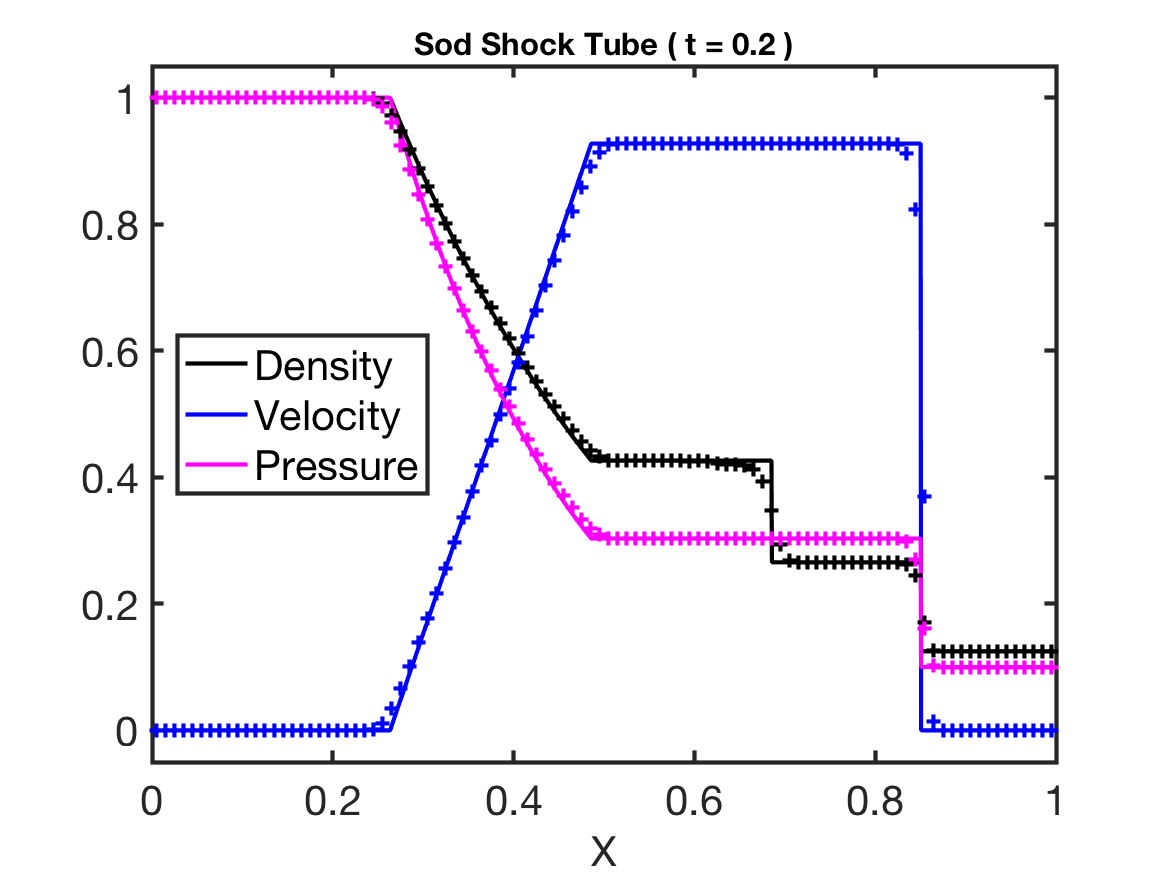
\includegraphics[width=18pc]{./Figures/Sod_Astronum_2018}
  \end{minipage}\hspace{0.5pc}%
  \begin{minipage}{18pc}
    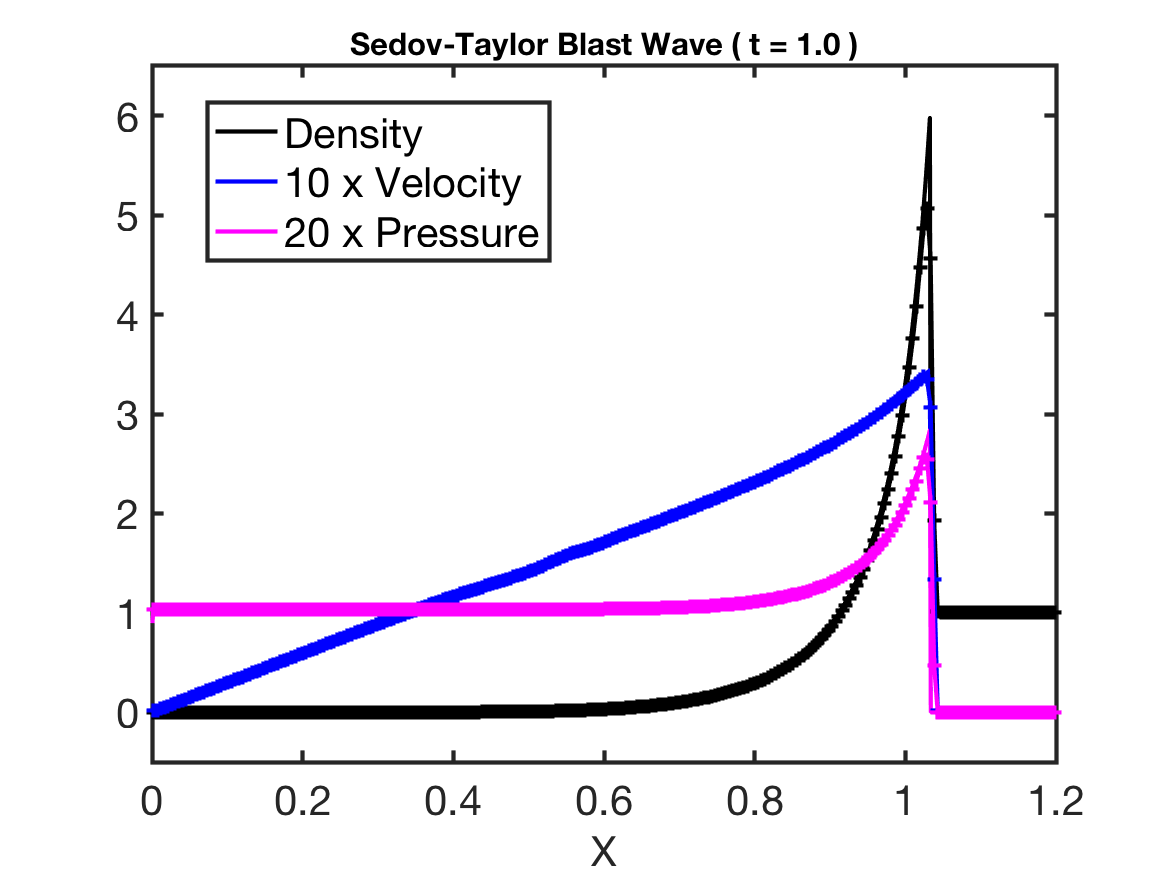
\includegraphics[width=18pc]{./Figures/Sedov_Astronum_2018}
  \end{minipage}
  \caption{\label{fig:SodSedov}{\it Left panel:} numerical solution of Sod's problem using $100$ elements (plusses) compared with the exact solution (solid lines; from \cite{toro_1999}).  {\it Right panel:} numerical solution of the Sedov-Taylor blast wave using $256$ elements (plusses) against the exact solution (solid lines).}
\end{figure}

\subsubsection{Sedov-Taylor blast wave}

This test, detailed in \cite{sedov_1959} (see also {\S}99 in \cite{landauLifshitz_1979}), is computed in spherical polar coordinates with the assumption of spherical symmetry.\footnote{In this paper, all tests in spherical polar coordinates are computed with the assumption of spherical symmetry.}
The computational domain is $D=[0,1.2]$, and the initial condition consists of a fluid at rest with density $\rho=1$.  
The adiabatic index is $\Gamma=1.4$, and an amount of thermal energy equal to $1$ is released in the innermost element.  
We use $256$ elements and run until $t=1$, using $C_{\TCI}=0.03$.  
Again, the DG method captures the characteristic of the exact solution.  
The maximum density in the shock is somewhat lower for the numerical solution than the exact value (about $5$ versus $6$).  

\subsubsection{Shu-Osher shock tube}

This test from \cite{shuOsher_1989} is suitable for measuring the amount of dissipation in a numerical scheme.  
The one-dimensional computational domain is $D=[-5,5]$, and a discontinuity is placed at $x^{1}=-4$, separating the states
\begin{equation*}
  \vect{U}_{\leftState}=\big( 3.857143, 10.14185, 0.0, 0.0, 39.16667 \big)^{\trans}\quad\text{and}\quad
  \vect{U}_{\rightState}=\big( 1+0.2\times\sin(5 x^{1}), \vect{0.0}, 2.5 \big)^{\trans},
\end{equation*}
where the adiabatic index is $\Gamma=1.4$.  
The density variations ahead of the Mach=3 shock are compressed through the shock and result in higher-frequency variations downstream, which can be difficult to capture with an excessively dissipative scheme.  

We run this test to $t=1.8$ using $200$ elements.  
In the two upper panels of Figure~\ref{fig:ShuOsher} we plot the density for various values of the troubled-cell indicator threshold $C_{\TCI}$; $0.0$ (full limiting, green), $0.03$ (magenta), $0.3$ (red), and $3.0$ (blue).  
Larger $C_{\TCI}$ implies less limiting.  
The results are compared with a reference solution computed with $2048$ elements.  
With full limiting, the scheme is unable to capture the density variations behind the shock (cf. upper right panel in Figure~\ref{fig:ShuOsher}).  
When $C_{\TCI}=0.03$, the variations are better resolved, but the amplitudes are much reduced relative to the reference solution.  
With $C_{\TCI}=3.0$, the variations are well resolved and the amplitudes are comparable to the reference.  
\begin{figure}[h]
  \centering
  \begin{minipage}{18pc}
    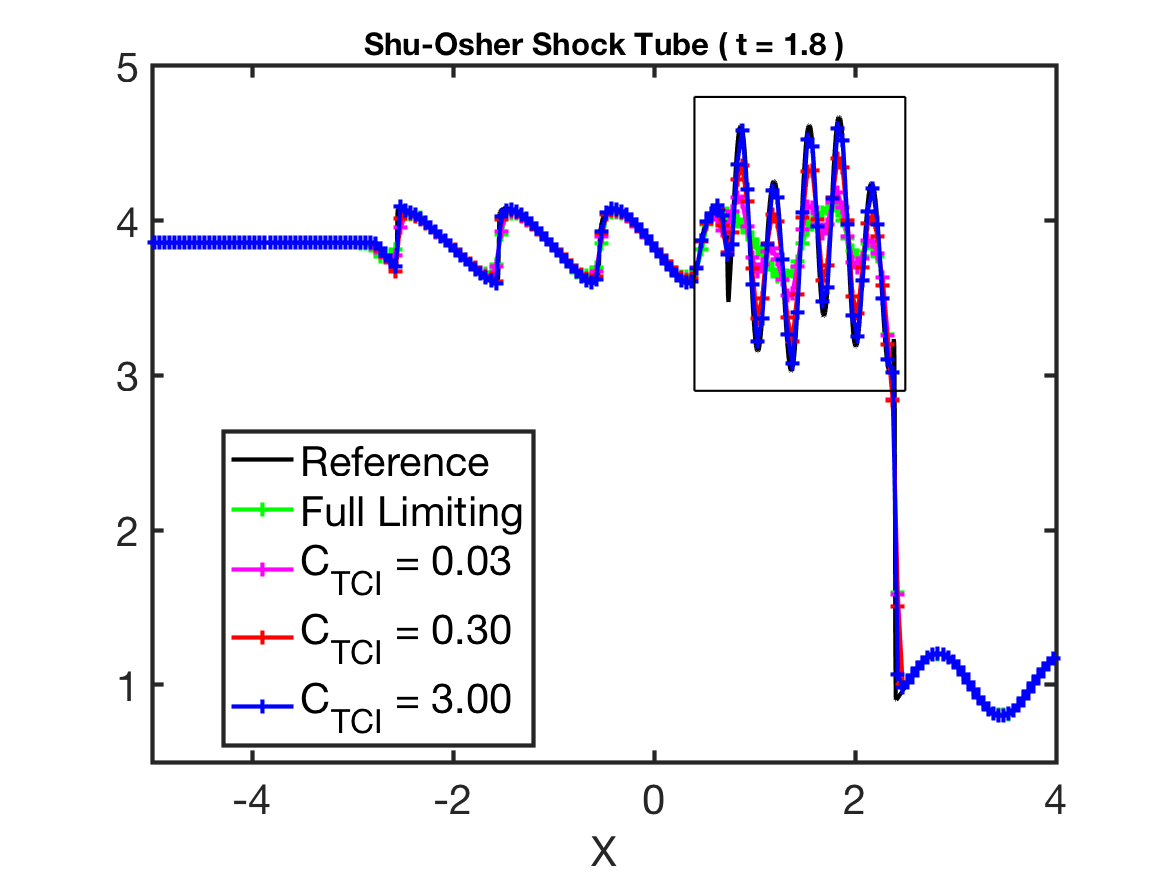
\includegraphics[width=18pc]{./Figures/ShuOsher_Astronum_2018}
  \end{minipage}\hspace{0.5pc}%
  \begin{minipage}{18pc}
    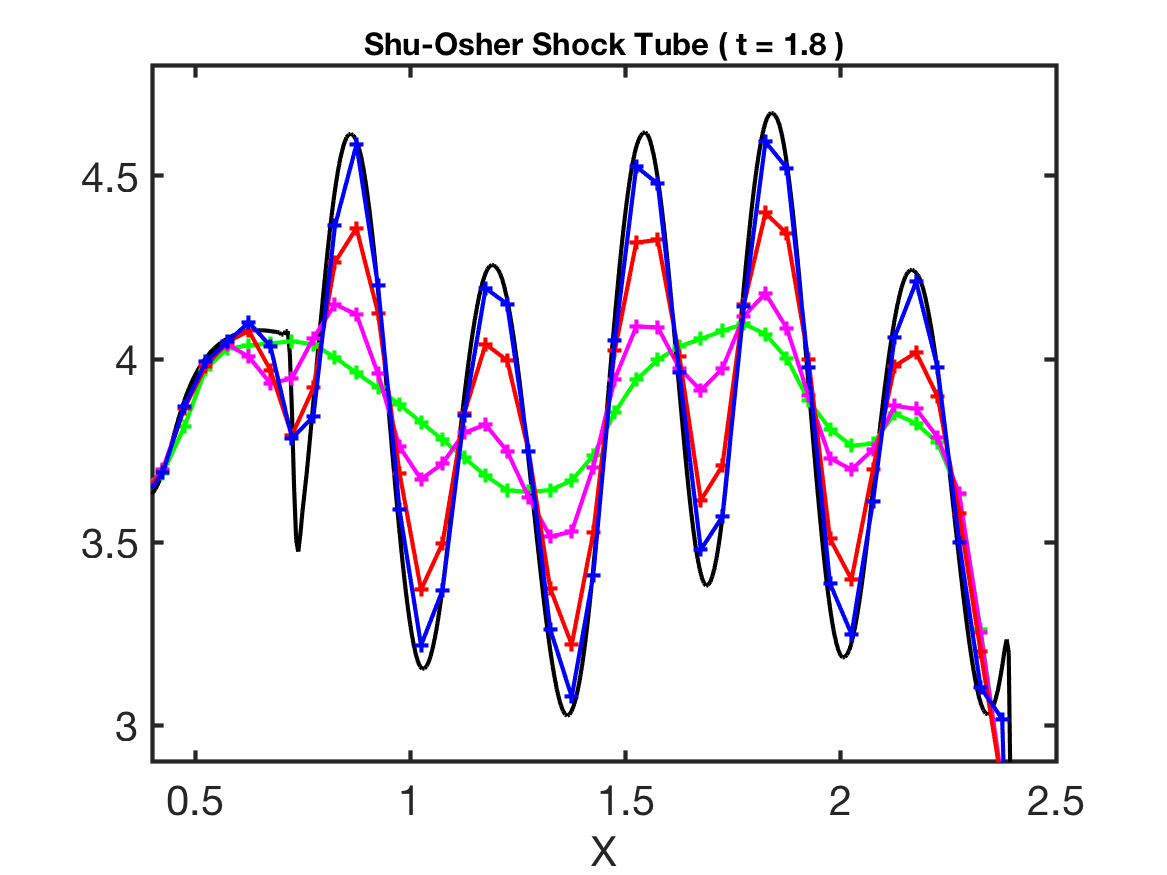
\includegraphics[width=18pc]{./Figures/ShuOsher_Inset_Astronum_2018}
  \end{minipage} \\
  \begin{minipage}{12pc}
    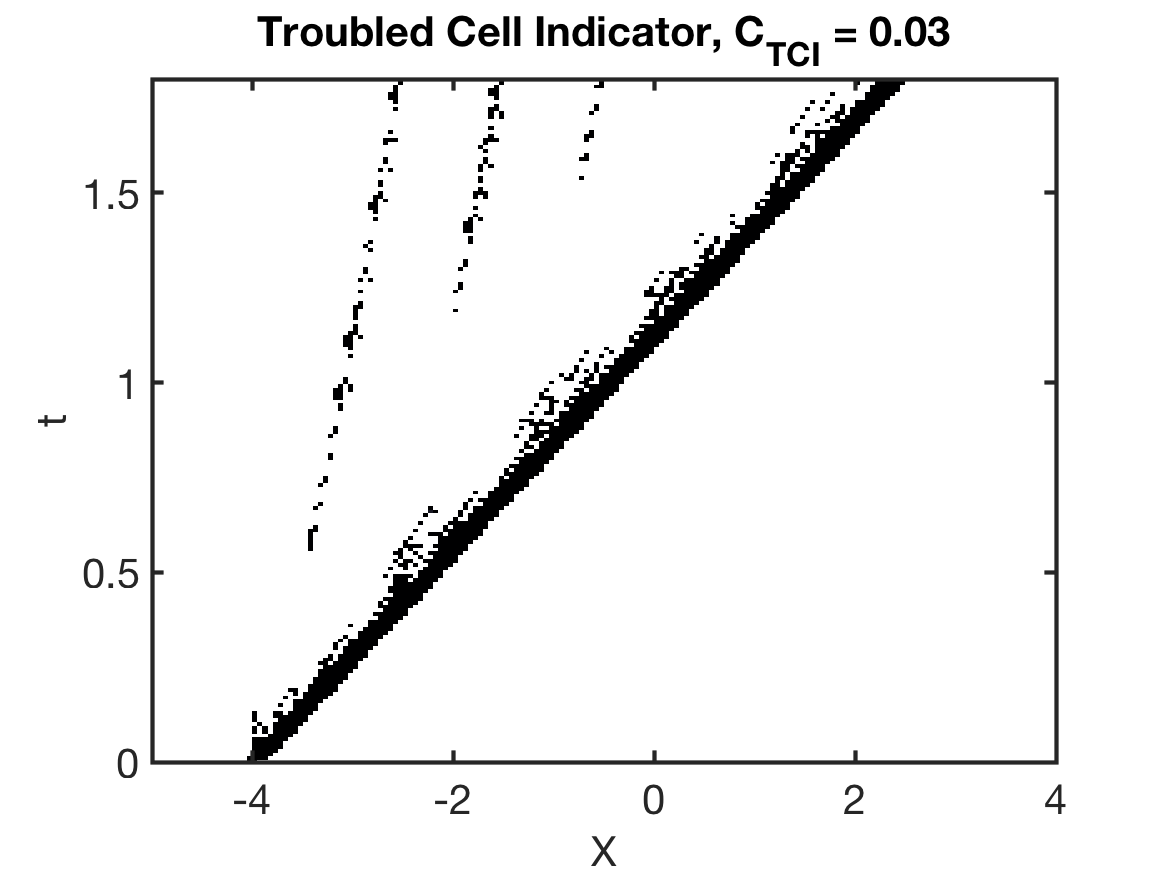
\includegraphics[width=12pc]{./Figures/ShuOsher_TCI_0015_Astronum_2018}
  \end{minipage}\hspace{0.5pc}%
  \begin{minipage}{12pc}
    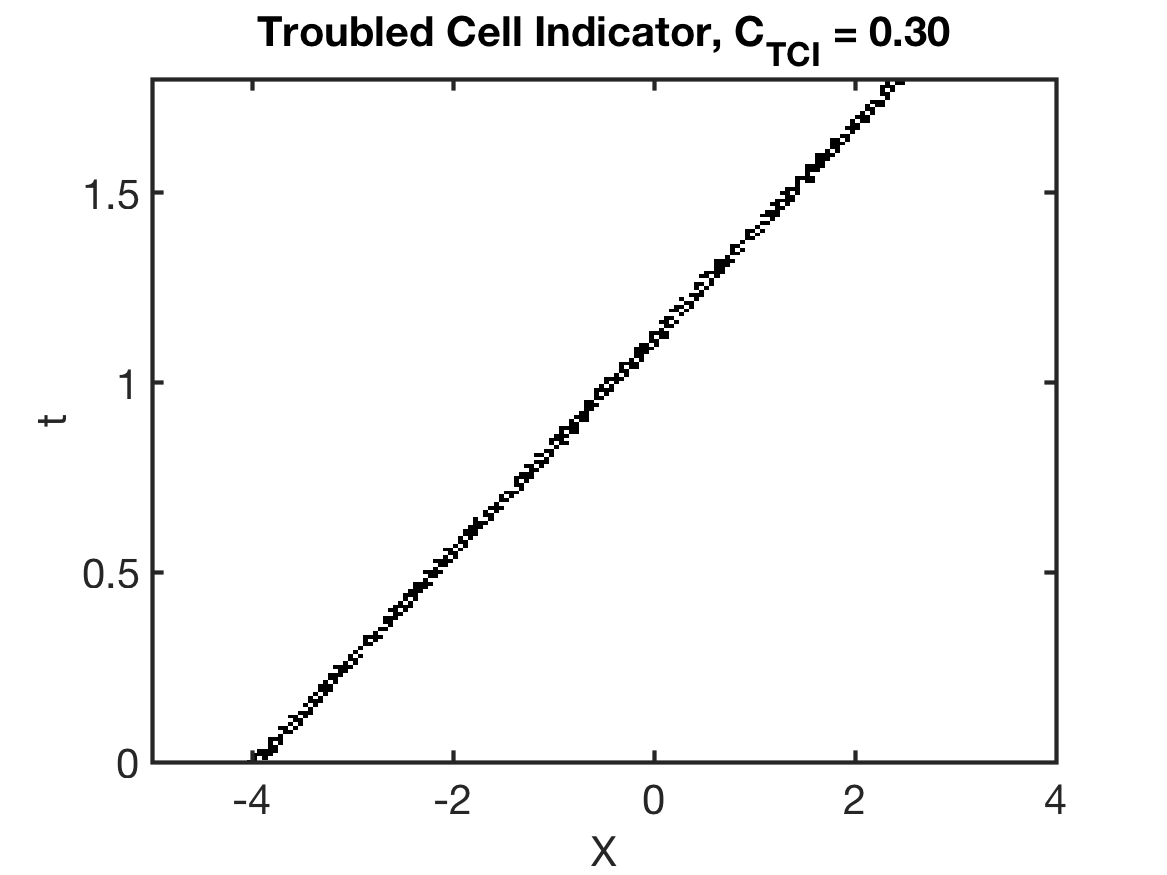
\includegraphics[width=12pc]{./Figures/ShuOsher_TCI_0150_Astronum_2018}
  \end{minipage}\hspace{0.5pc}
  \begin{minipage}{12pc}
    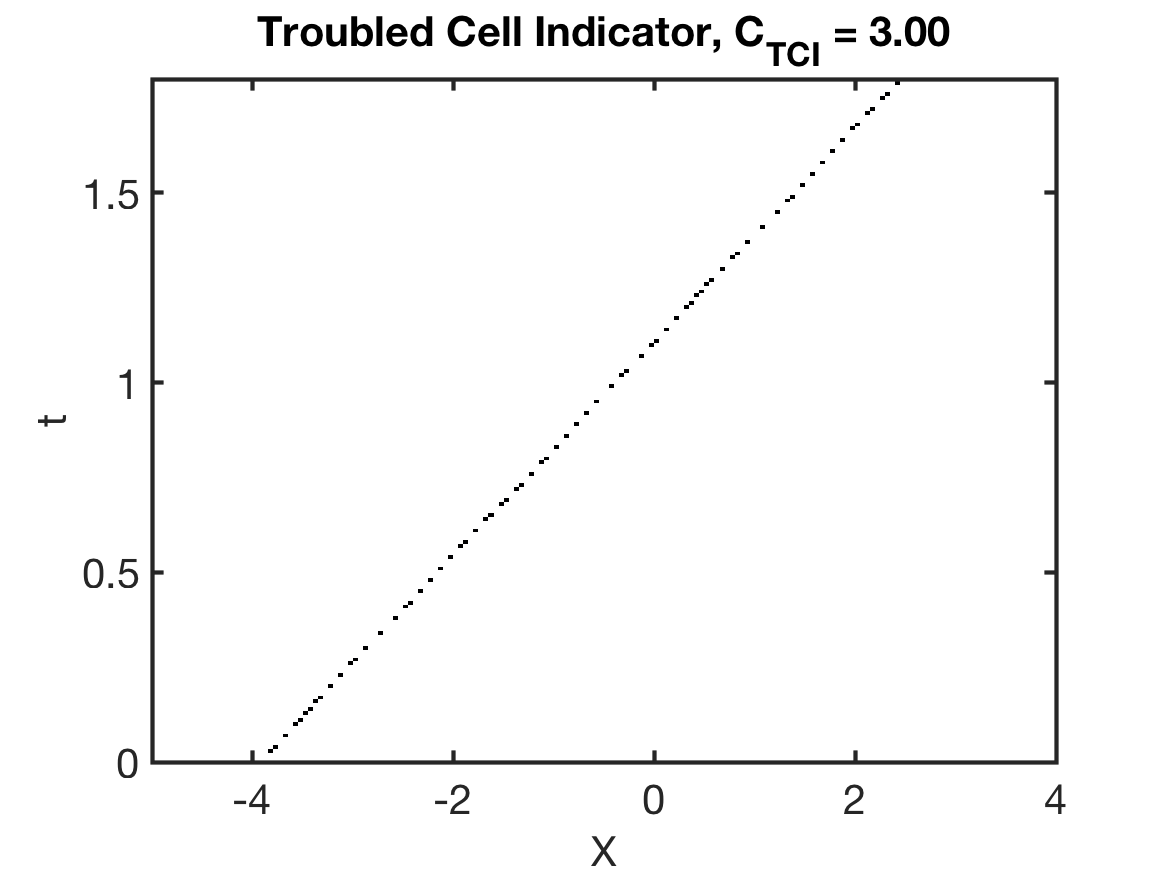
\includegraphics[width=12pc]{./Figures/ShuOsher_TCI_1500_Astronum_2018}
  \end{minipage}
  \caption{\label{fig:ShuOsher}Results for the Shu-Osher shock tube problem computed with $200$ elements.  The upper panels show the mass density at $t=1.8$ for various values of the troubled-cell indicator threshold $C_{\TCI}$, compared with a high-resolution (2048 elements) reference solution.  In the lower panels we show elements flagged for limiting in the $xt$-plane for various values of $C_{\TCI}$.}
\end{figure}
In the lower panels of Figure~\ref{fig:ShuOsher} we plot locations in the $xt$-plane of elements flagged for limiting by the troubled-cell indicator: $C_{\TCI}=0.03$ (left), $C_{\TCI}=0.3$ (middle), and $C_{\TCI}=3.0$ (right).  
With $C_{\TCI}=0.03$, limiting is triggered in a wide region around the shock and around the peaks of the three leftmost density variations in the upper left panel in Figure~\ref{fig:ShuOsher}.  
With $C_{\TCI}=3.0$, limiting is only triggered in the shock.  

\subsubsection{Kelvin-Helmholtz (KH) instability}
This hydrodynamic instability is of significant astrophysical relevance --- including during the explosion phase of CCSNe --- and may occur in the interface separating fluids in relative motion.  
We compute this problem on the unit square $D=[0,1]\times[0,1]$, imposing periodic boundary conditions, and with initial conditions and single-mode perturbations taken from \cite{mcnally_etal_2012}.  
We use $256^{2}$ elements and evolve until $t=3.0$, well into the nonlinear regime.  
Results are displayed in Figure~\ref{fig:KelvinHelmholtz}.  
We have computed two models, one with $C_{\TCI}=0.06$ (left panels) and one without limiting ($C_{\TCI}\to\infty$; right panels).  

\begin{figure}[h]
  \centering
  \begin{minipage}{18pc}
    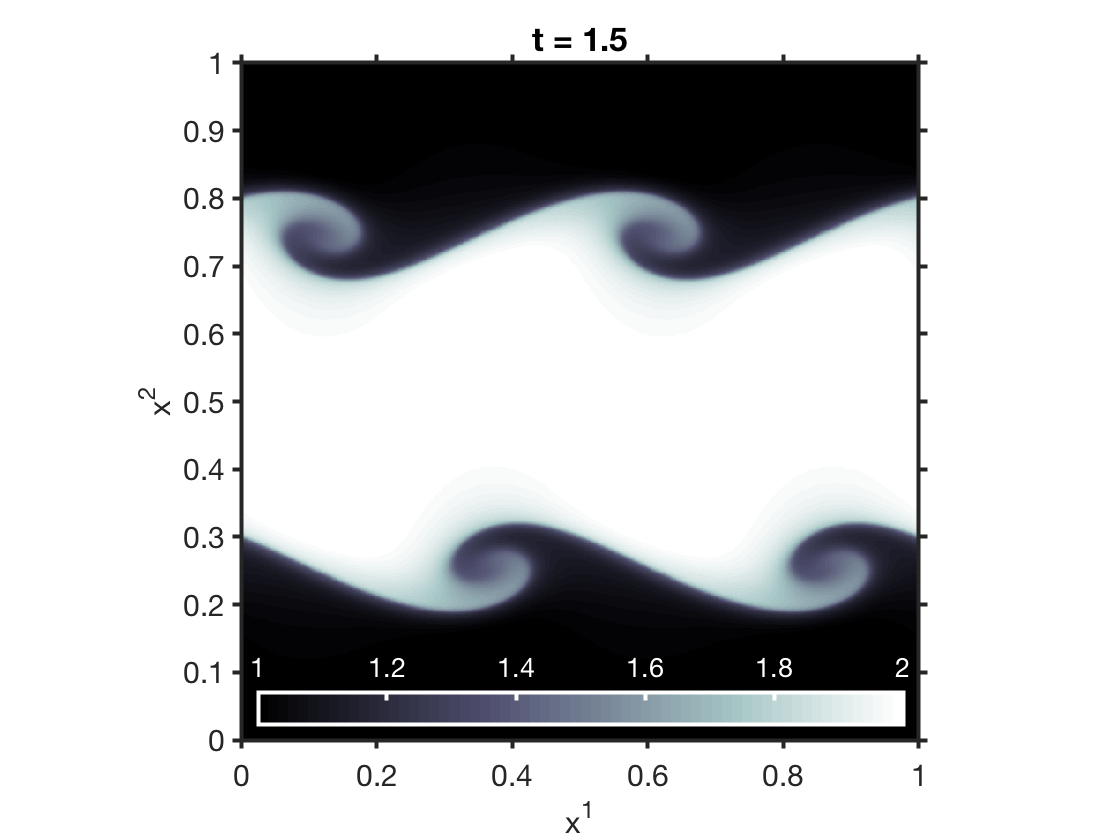
\includegraphics[width=18pc]{./Figures/KelvinHelmholtz_15_Astronum_2018}
  \end{minipage}\hspace{0.5pc}
  \begin{minipage}{18pc}
    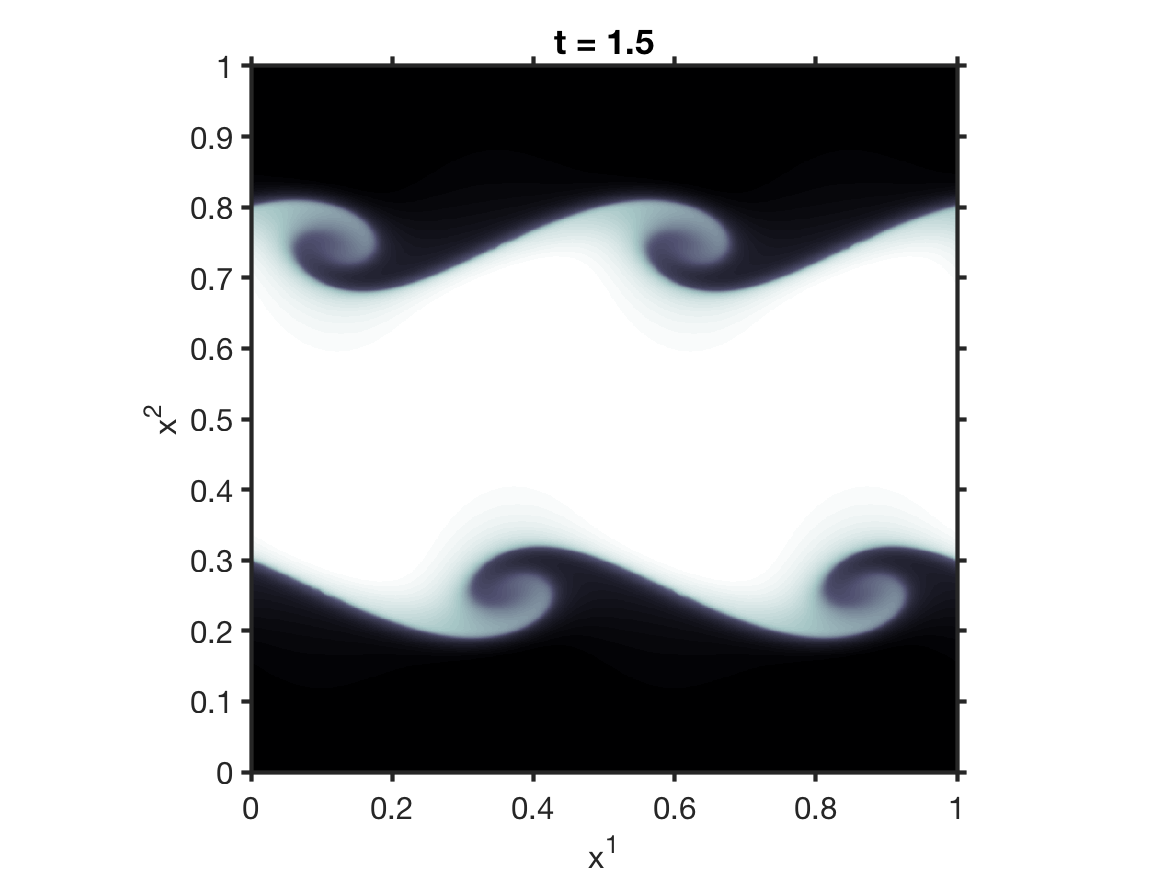
\includegraphics[width=18pc]{./Figures/KelvinHelmholtz_15_noLim_Astronum_2018}
  \end{minipage} \\
  \begin{minipage}{18pc}
    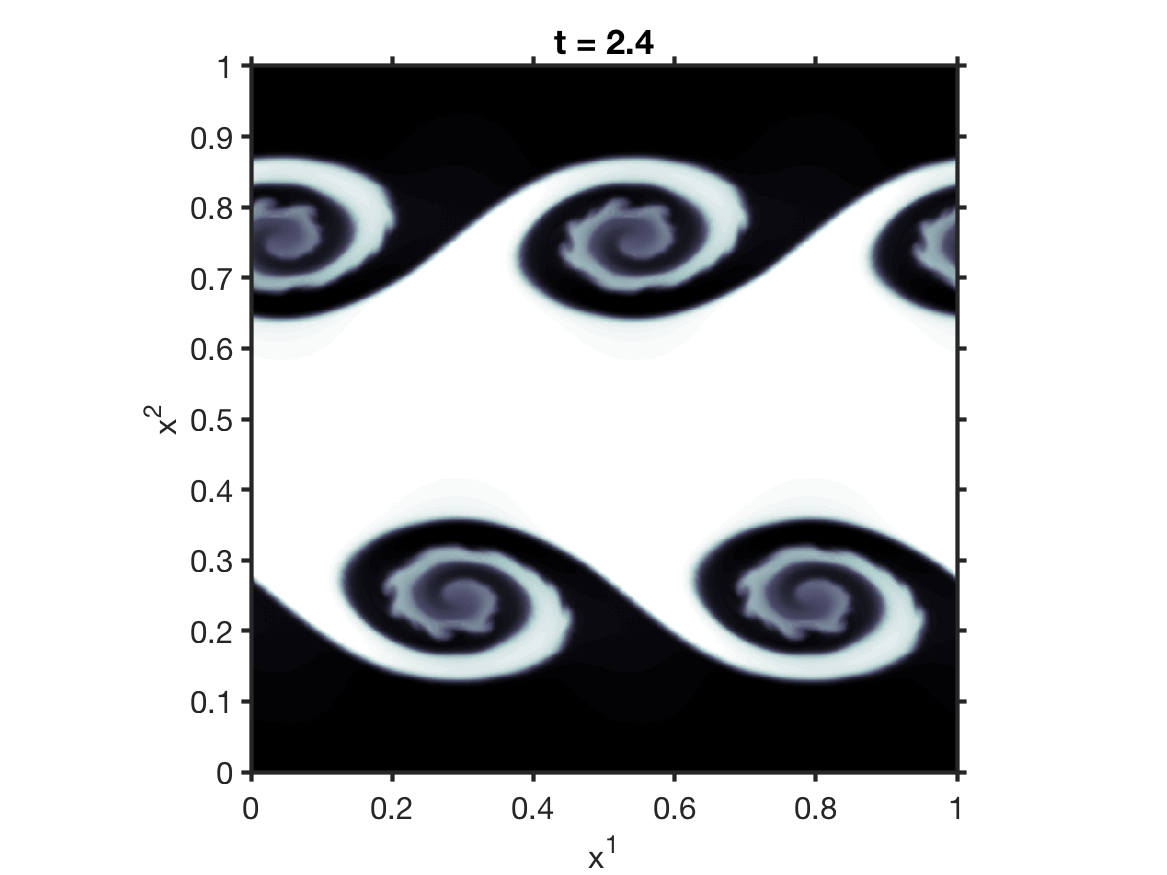
\includegraphics[width=18pc]{./Figures/KelvinHelmholtz_24_Astronum_2018}
  \end{minipage}\hspace{0.5pc}
  \begin{minipage}{18pc}
    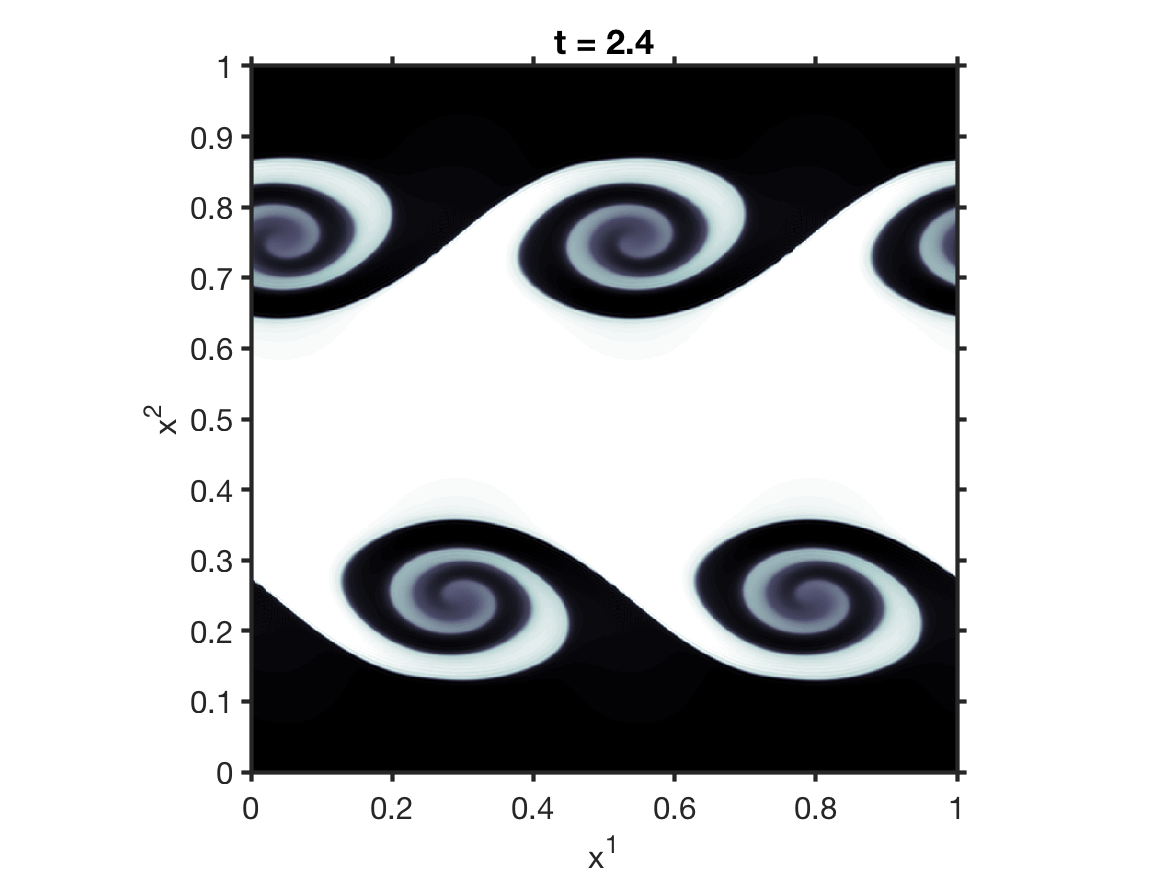
\includegraphics[width=18pc]{./Figures/KelvinHelmholtz_24_noLim_Astronum_2018}
  \end{minipage} \\
  \begin{minipage}{18pc}
    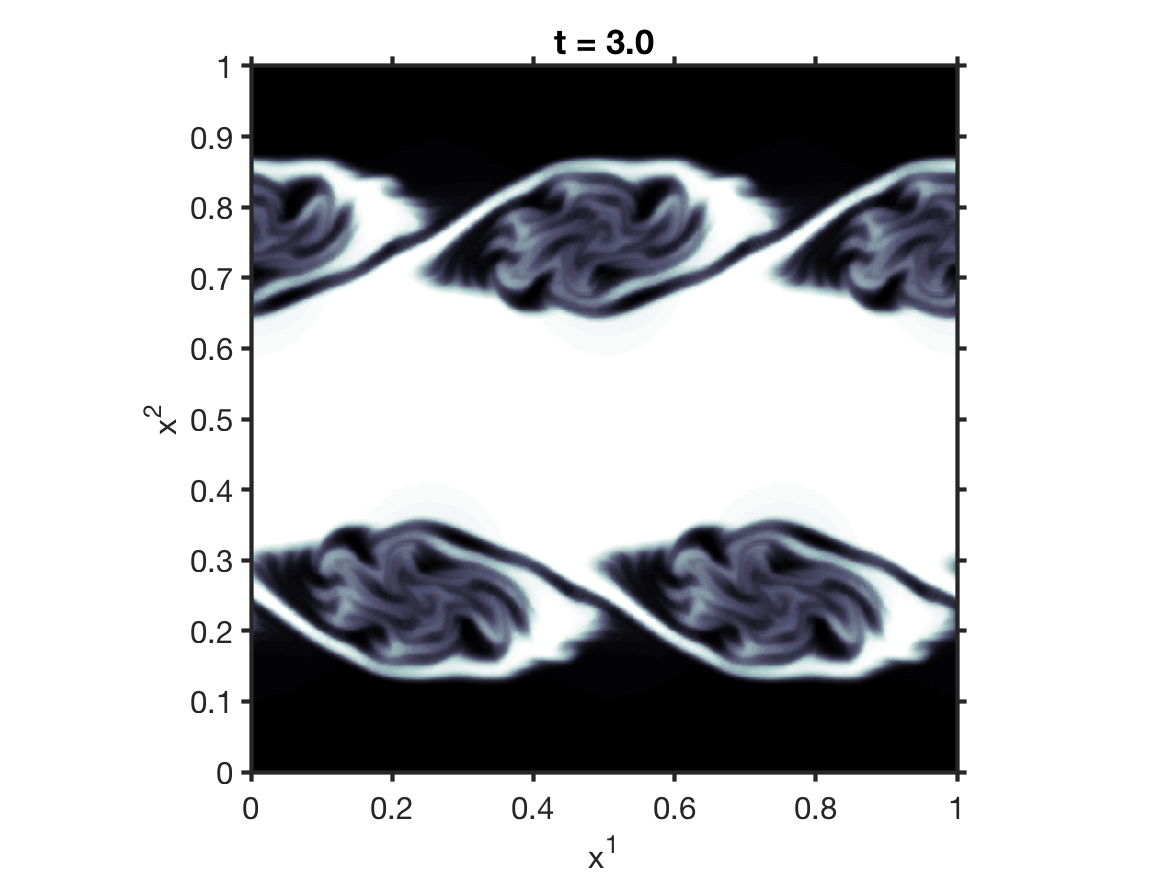
\includegraphics[width=18pc]{./Figures/KelvinHelmholtz_30_Astronum_2018}
  \end{minipage}\hspace{0.5pc}
  \begin{minipage}{18pc}
    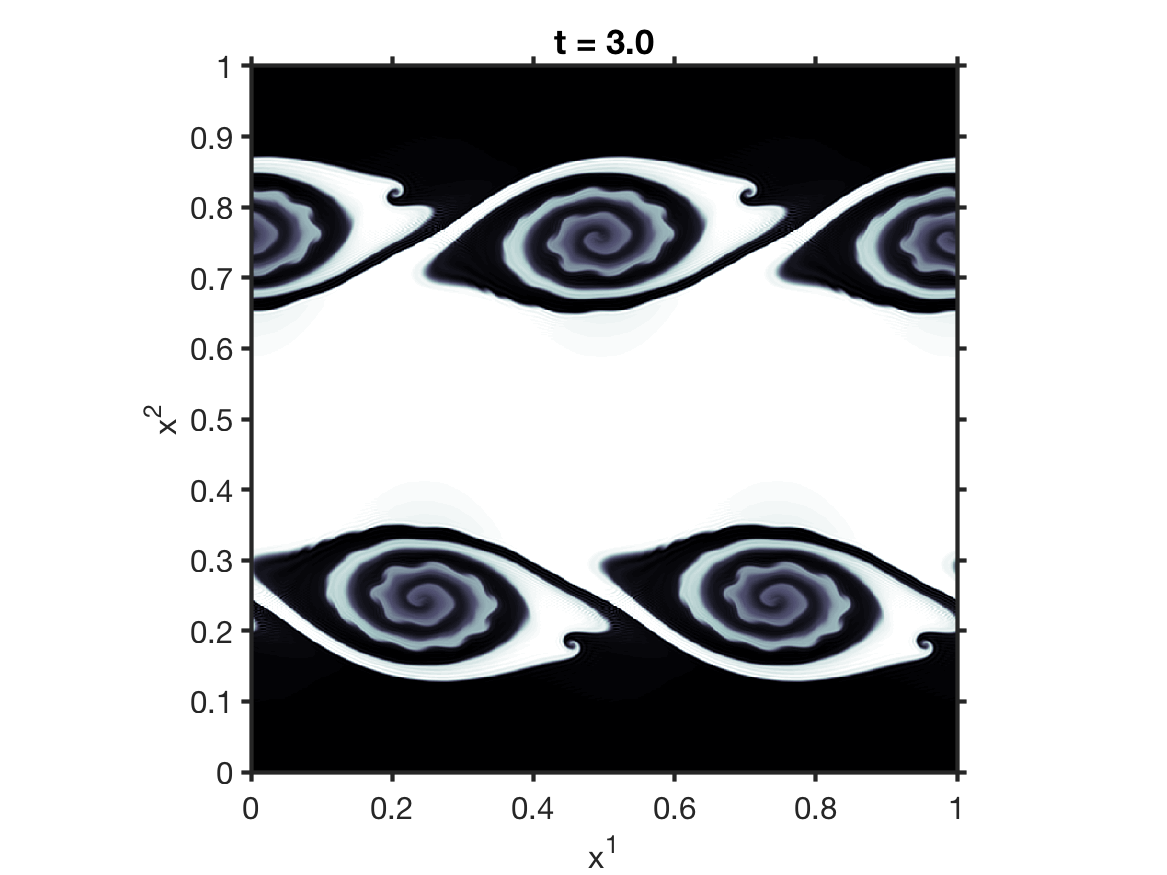
\includegraphics[width=18pc]{./Figures/KelvinHelmholtz_30_noLim_Astronum_2018}
  \end{minipage}
  \caption{\label{fig:KelvinHelmholtz}Mass density from the KH instability at various times, computed with $256^{2}$ elements: $t=1.5$ (top panels), $t=2.4$ (middle panels), and $t=3.0$ (bottom panels).  Results for $C_{\TCI}=0.06$ and $C_{\TCI}\to\infty$ (no limiting) are shown in the left and right panels, respectively.}
\end{figure}

Early on ($t=1.5$), the results from the two runs are practically indistinguishable, show no sign of developing secondary billows, and agree visually with results presented in \cite{mcnally_etal_2012}.  
When $t=2.4$, the run with $C_{\TCI}=0.03$ has started to develop secondary billows within the coiled-up interface separating dense (white) and less dense (black) fluids, while the model with no limiting has not.  
When $t=3.0$, these secondary instabilities appear to have largely destroyed the coil structure for the model with limiting, while the coils remain intact in the model without limiting (although secondary billows have started to form in this model at this time).  
As discussed in more detail by \cite{mcnally_etal_2012}, the development of the secondary billows may be an artifact of numerical perturbations and diffusion, which is delayed when the resolution is increased.  
Our results are consistent with this in the sense that the less diffusive model develops secondary billows later.  

\subsubsection{Liska-Wendroff implosion}

This test from \cite{liskaWendroff_2003} is computed on a 2D domain $D=[0,0.3]\times[0,0.3]$ with reflecting boundary conditions using $256^{2}$ elements.  
Below the line $x^{2}=0.15-x^{1}$, we initially set $\vect{U}=\big(0.125,\vect{0.0},0.35\big)^{\trans}$, while $\vect{U}=\big(1.0,\vect{0.0},2.5\big)^{\trans}$ elsewhere.  

\begin{figure}[h]
  \centering
  \begin{minipage}{18pc}
    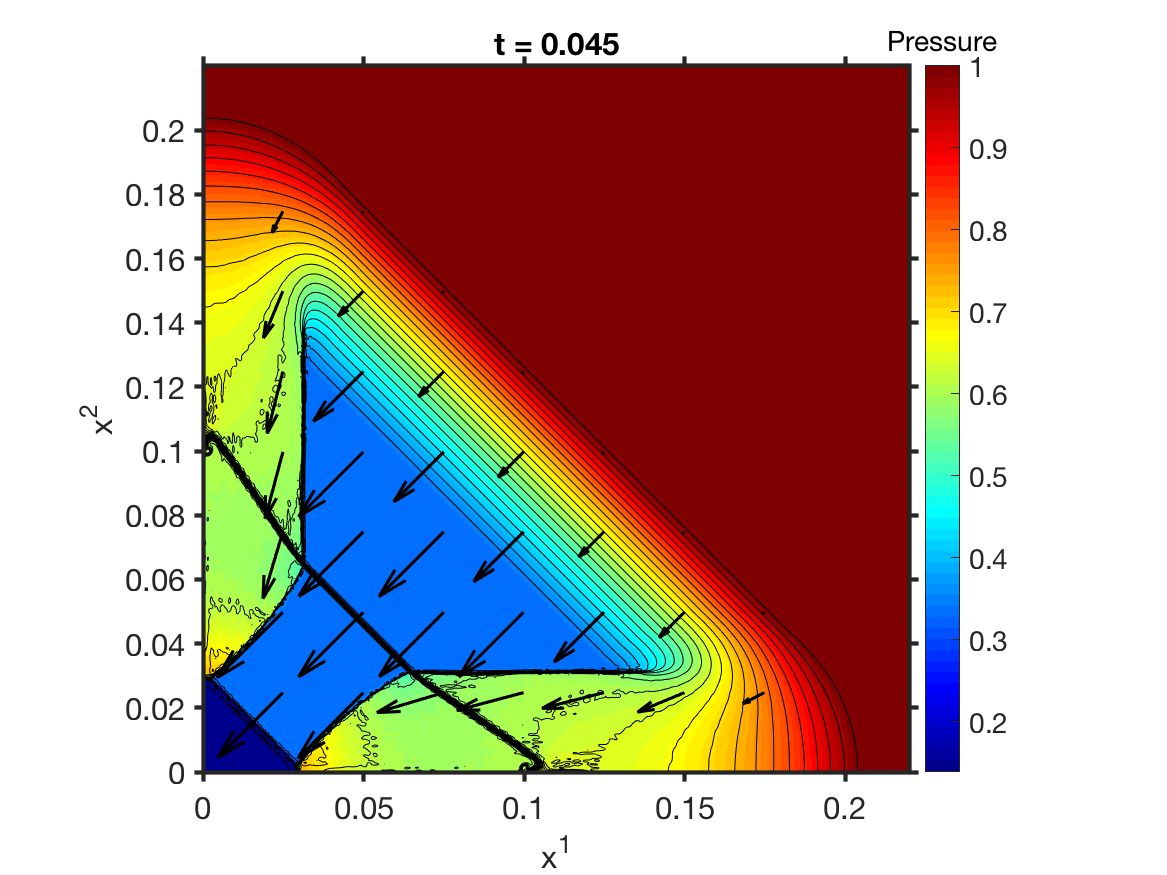
\includegraphics[width=18pc]{./Figures/Implosion_01_HighTCI_Astronum_2018}
  \end{minipage}\hspace{0.5pc}%
  \begin{minipage}{18pc}
    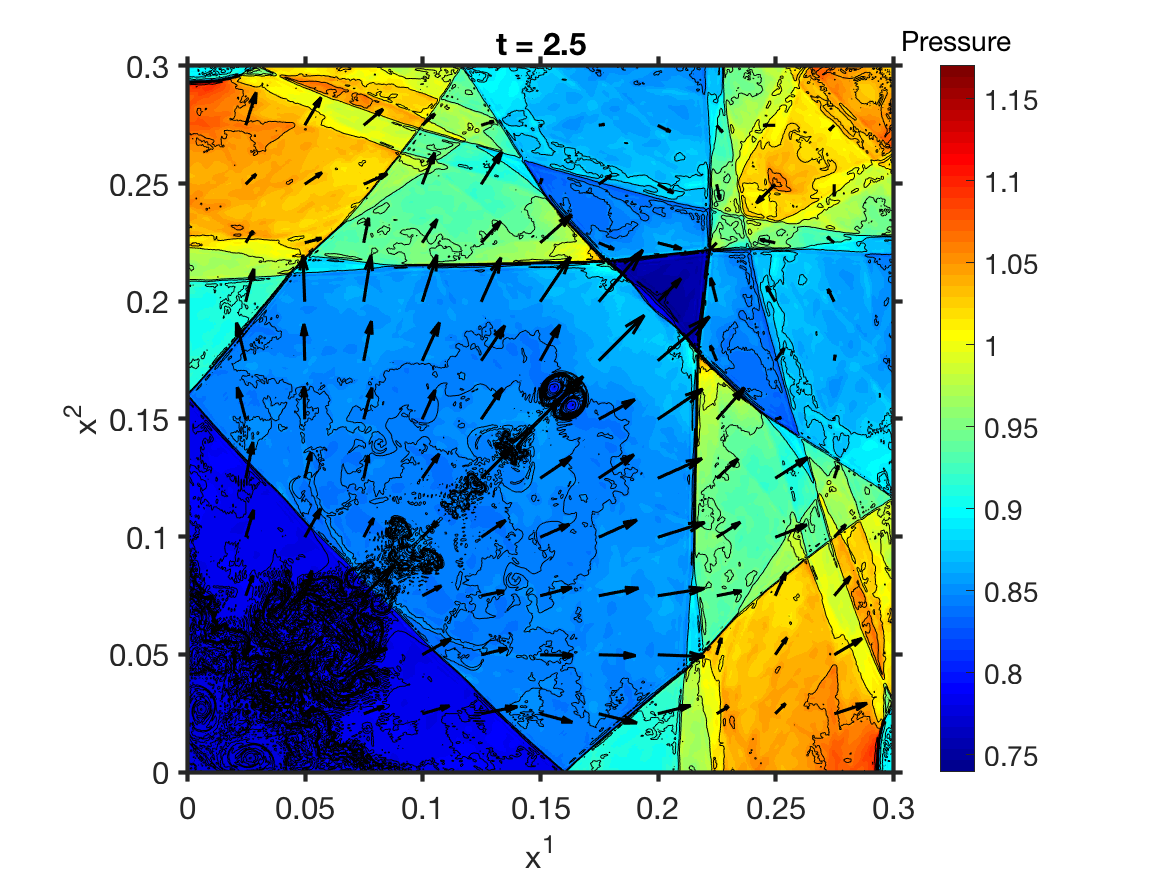
\includegraphics[width=18pc]{./Figures/Implosion_02_HighTCI_Astronum_2018}
  \end{minipage}
  \caption{\label{fig:Implosion}Plots for the Liska-Wendroff implosion problem at $t=0.045$ (left) and $t=2.5$ (right), intended to match Figures~4.10 and 4.11 in \cite{liskaWendroff_2003}.  The color map shows the pressure distribution, black contours show the mass density, while arrows indicate the velocity.}
\end{figure}

Results for $t=0.045$ and $t=2.5$, with $C_{\TCI}=0.6$, are displayed in Figure~\ref{fig:Implosion} (left and right panels, respectively), which agree qualitatively with \cite{liskaWendroff_2003}, who compared the results of eight different schemes for this problem.  
When $t=0.045$, a shock wave propagates towards the origin of $D$, while a contact discontinuity is trailing the shock (cf. density contours), and a rarefaction wave is spreading in the opposite directions.  
When $t=2.5$, a complex flow pattern with multiple shocks has emerged due to multiple reflections off the boundaries.  
The initial symmetry about the $x^{1}=x^{2}$ diagonal is maintained, and the results from \thornado\ agree qualitatively with the unsplit schemes in \cite{liskaWendroff_2003}.  
In the right panel of Figure~\ref{fig:Implosion}, the chatacteristic ``jet'' has formed and propagates along the diagonal, similar to that displayed by CLAW and WENO in \cite{liskaWendroff_2003}.  

\subsubsection{Standing accretion shock (SAS)}

This test is of immediate relevance to simulation of CCSNe.  
The initial conditions, described in detail in \cite{blondin_etal_2003}, have been used by many to study the standing accretion shock instability (SASI) and CCSN explosion dynamics.  
We follow closely the description in \cite{blondin_etal_2003} to initialize this test.  
We use spherical polar coordinates, let $D=[0.2,2.0]$, and $\Gamma=4/3$.  
The gravitational potential is given by the point-mass formula with $GM=0.5$.  
A stationary shock is placed at a radius $R_{\shock}=1$.  
Ahead of the shock, the flow is essentially in free-fall towards the shock with a constant Mach number of $100$.  
The mass accretion rate is held fixed at the outer boundary to $\dot{M}=4\pi$.  
Below the shock, $r\in[0.2,1]$, the settling solution is obtained by solving Bernoulli's equation.  
Matter flows through the inner boundary, and the density and pressure in boundary elements are set by extrapolating from $D$ assuming $\rho\propto r^{-3}$ and $E\propto r^{-4}$, while the momentum components are held fixed to their initial values.  

\begin{figure}[h]
  \centering
  \begin{minipage}{18pc}
    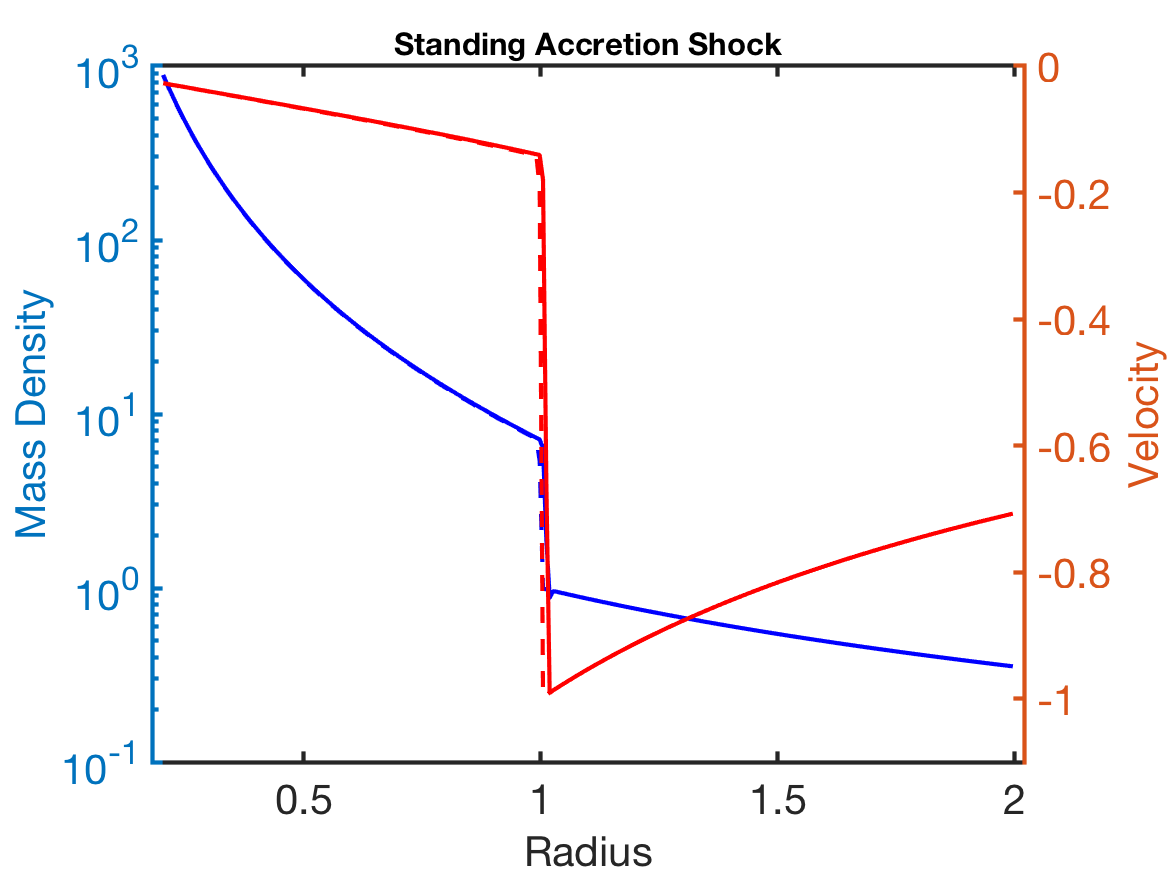
\includegraphics[width=18pc]{./Figures/SAS_Astronum_2018}
  \end{minipage}\hspace{0.5pc}%
  \begin{minipage}{18pc}
    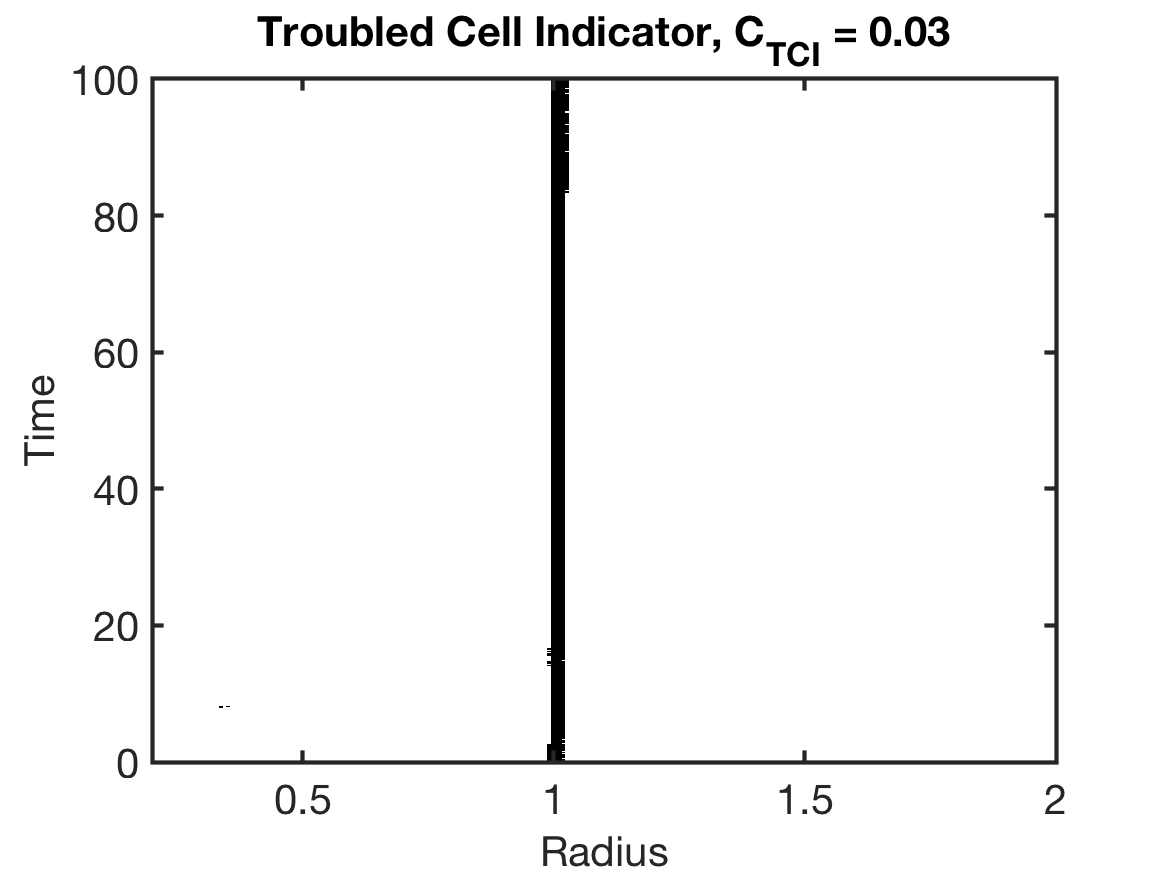
\includegraphics[width=18pc]{./Figures/SAS_TCI_Astronum_2018}
  \end{minipage} \\
  \begin{minipage}{36pc}
    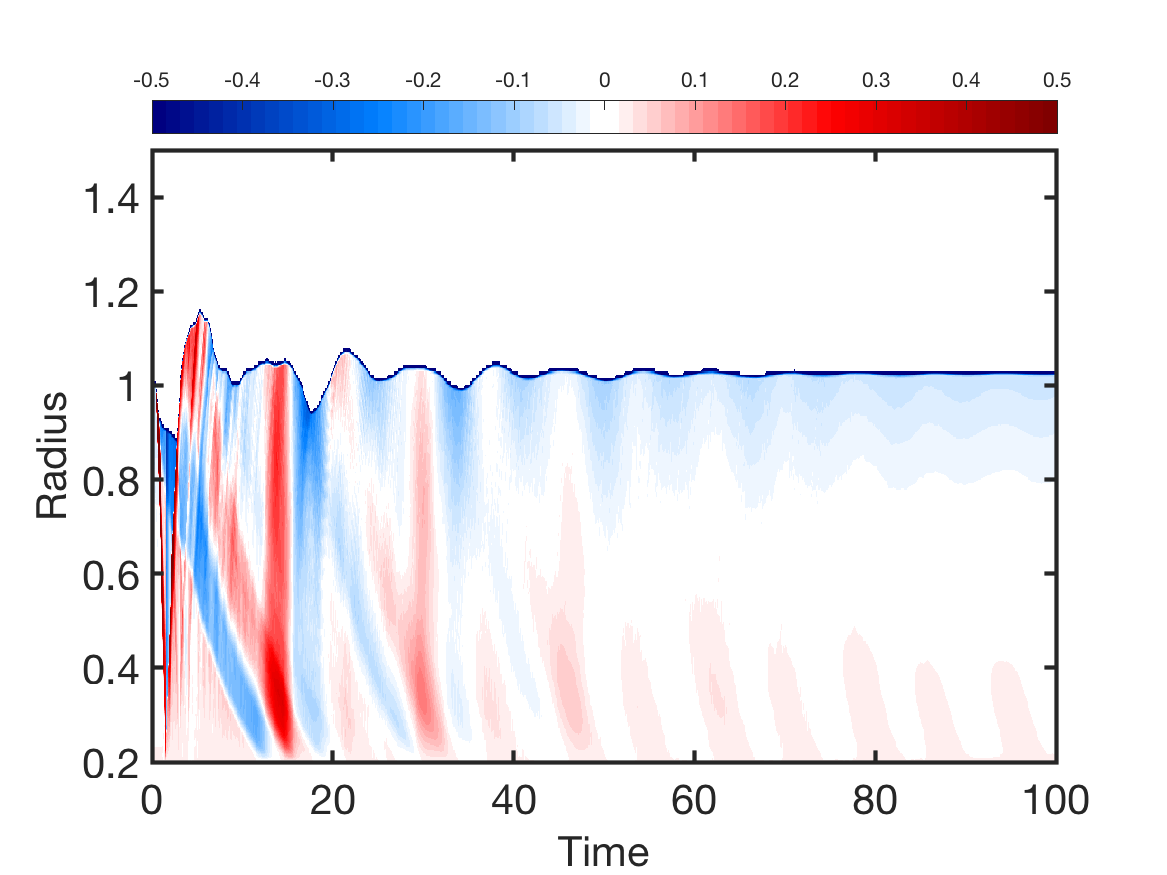
\includegraphics[width=36pc]{./Figures/SAS_Perturbed_Astronum_2018}
  \end{minipage}
  \caption{\label{fig:SAS}Results from the SAS test using $256$ elements.  In the upper left panel we plot the mass density (blue) and velocity (red) versus radius for the initial condition (dashed lines) and for $t=100$ (solid lines) from an unperturbed run.  In the upper right panel we show elements flagged for limiting in the $rt$-plane.  In the bottom panel we show results from a perturbed model, where we plot the relative deviation of the pressure below the shock; cf. Eq.~\eqref{eq:pressureDeviation}.}
\end{figure}

We use $256$ elements and run the tests until $t=100$ ($>5$ dynamical times \cite{blondin_etal_2003}).  
Results are shown in Figure~\ref{fig:SAS}.  
In the first test we show results from an unperturbed run to gauge the ability of the DG method to maintain the initial state.  
In the upper left panel we compare the initial state (dashed lines) with the solution at $t=100$.  
Except for a slight shift ($\sim1\%$) in the position of the shock, the initial and final states are indistinguishable on the plot.  
Also, there are no oscillations visible in the numerical results.  
In the upper right panel we show elements flagged for limiting in the $rt$-plane (we set $C_{\TCI}=0.03$ in this run), which illustrates how limiting is confined to the shock.  
In the second test we placed a shell with thickness $0.2$ and density three times higher than the ambient density ahead of the shock to induce a strong radial perturbation (similar to \cite{blondin_etal_2003}; see their Figure~4).  
The initial condition is stable against radial perturbations.  
In the lower panel in Figure~\ref{fig:SAS} we plot the pressure deviation below the shock, defined as
\begin{equation}
  \delta p = (p-\bar{p})/\bar{p},
  \quad\text{where}\quad
  \bar{p}=p_{0}(r_{0}/r)^{4},
  \label{eq:pressureDeviation}
\end{equation}
and $p_{0}$ and $r_{0}$ are the pressure and radius at the inner boundary.  
As the shell falls through the shock, the strong perturbation results in an interesting pattern of waves propagating inside the shocked cavity, and oscillations of the shock position.  
The configuration eventually settles down to a configuration that is close to the initial condition (although the position of the shock is slightly larger than that of the initial state.)  

\subsubsection{Yahil-Lattimer collapse}

The final test of the NR hydrodynamics in \thornado\ involves self-gravity and is due to \cite{yahilLattimer_1982,yahil_1983}.  
It models the self-similar collapse of a polytropic star; i.e., $p=\kappa\rho^{\Gamma}$, where $\kappa$ is the polytropic constant.  
This test is also of immediate relevance to CCSN simulations.  
In \cite{yahilLattimer_1982,yahil_1983}, self-similar solutions to the gravitational collapse problem were constructed for $6/5\le\Gamma<4/3$.   
The solutions smoothly connect an homologously collapsing subsonic inner core (velocity proportional to radius) to a supersonically collapsing outer core in near free-fall ($u\propto r^{-1/2}$).  
\begin{figure}[h]
  \centering
  \begin{minipage}{18pc}
    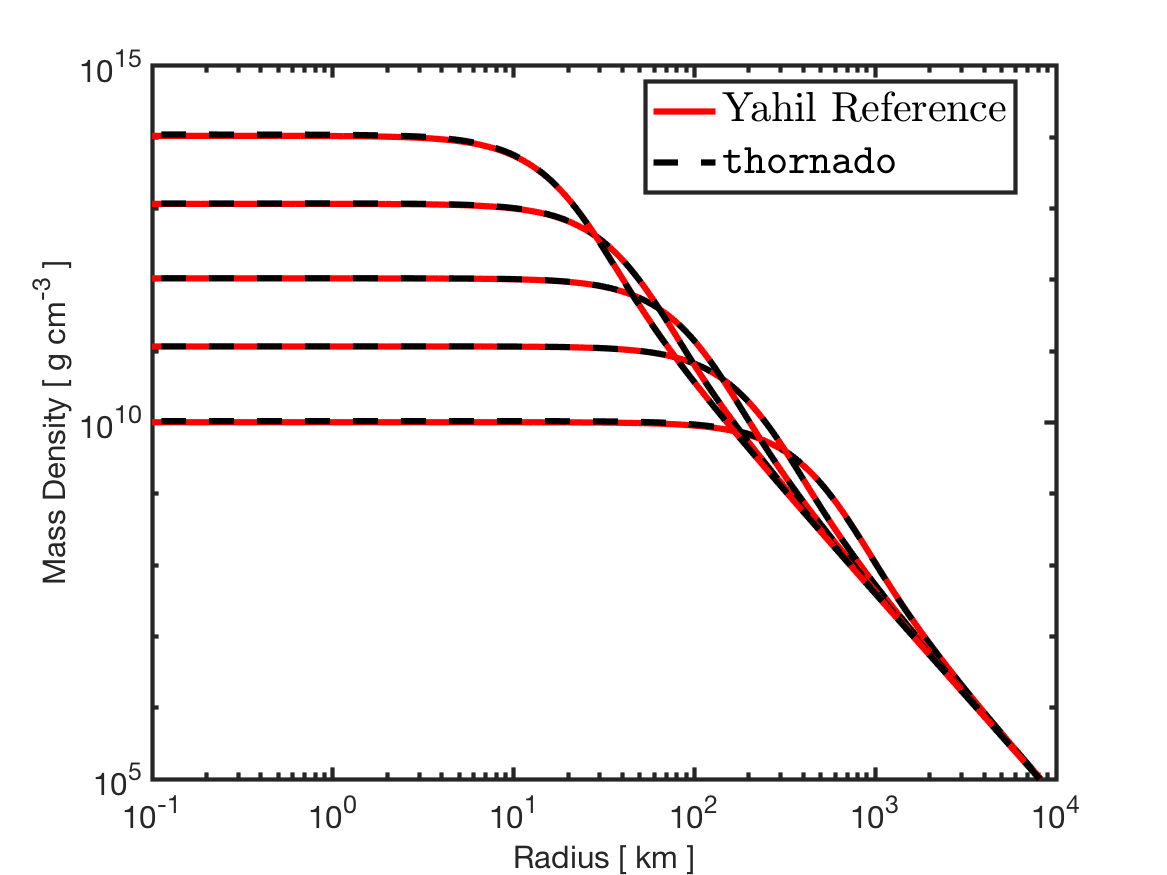
\includegraphics[width=18pc]{./Figures/YahilLattimerCollapse_MassDensity_Astronum_2018}
  \end{minipage}\hspace{0.5pc}%
  \begin{minipage}{18pc}
    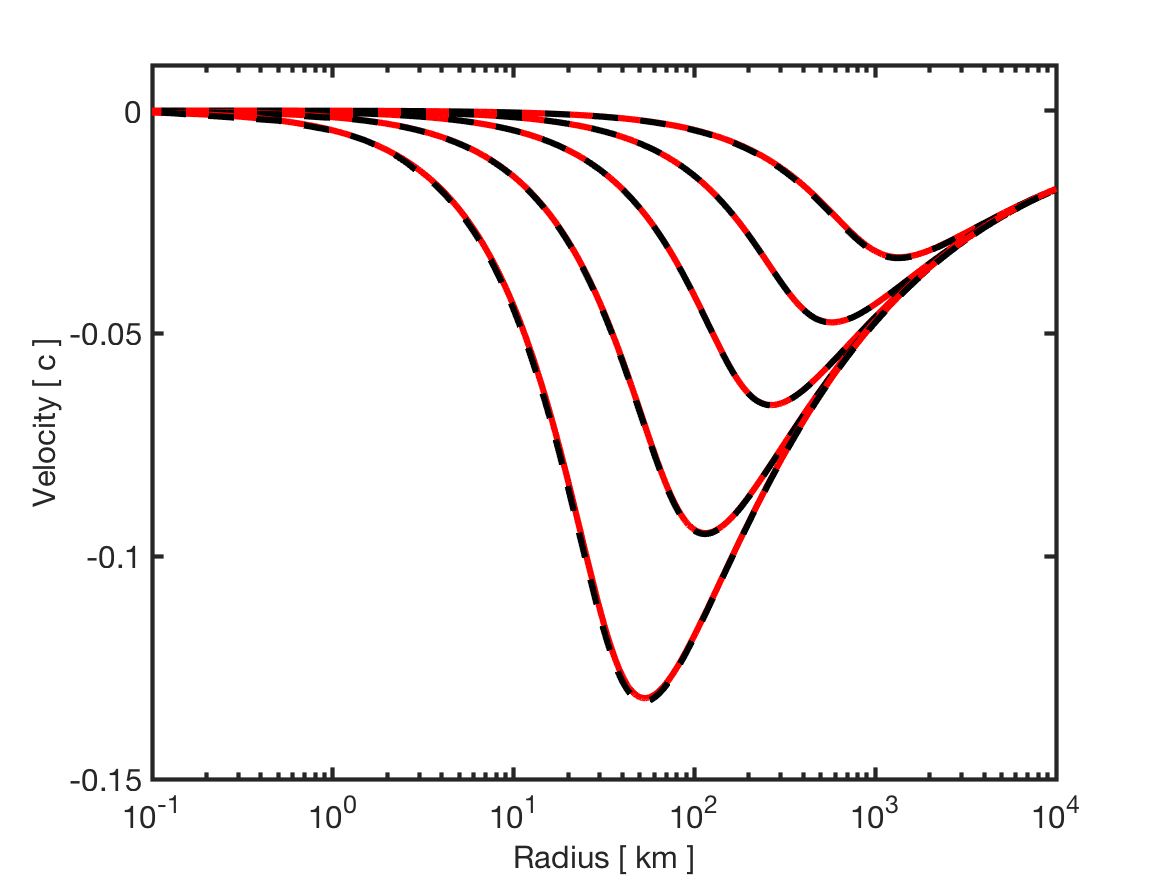
\includegraphics[width=18pc]{./Figures/YahilLattimerCollapse_Velocity_Astronum_2018}
  \end{minipage}
  \caption{\label{fig:YahilLattimer}Results from the Yahil-Lattimer collapse test using $256$ elements.  Results obtained with \thornado\ (dashed black) are compared with the reference solution from Yahil \cite{yahil_1983} (solid red).  The mass density (left panel) and velocity (right panel) are plotted versus radius.  We compare the solutions at select central densities during collapse, approximately $[10^{10},10^{11},10^{12},10^{13},10^{14}]$~g~cm$^{-3}$, which correspond to $(-t)=[51.0,15.0,5.0,1.5,0.5]$~ms.  }
\end{figure}
With two dimensional parameters in the model (the gravitational constant $G$ and the polytropic constant $\kappa$), the dimensionless similarity variable is
\begin{equation}
  X = \kappa^{-1/2} \, G^{(\Gamma-1)/2} \, r \, (-t)^{\Gamma-2},
\end{equation}
where the origin of time is the moment of infinite central density.  
All the hydrodynamic variables can be expressed as a function of $X$, and the time-dependent Euler equations can be recast as a system of ODEs (see \cite{yahil_1983} for details).  
To construct a reference to compare with our numerical results we have solved the ODEs given in \cite{yahil_1983} to obtain these self-similar solutions.  

We show results for a model with $\Gamma=1.30$.  
We use spherical polar coordinates, and let $D=[0,1\times10^{5}]$~km, which is covered with $256$ elements.  
The Newtonian gravitational potential is obtained by solving Poisson's equation using a third-order accurate continuous finite element method (e.g., \cite{brennerScott_2008}).  
We use a geometric grid to resolve the mass distribution as the star collapses and the central density increases from about $10^{9}$~g~cm$^{-3}$ to about $10^{14}$~g~cm$^{-3}$.  
The size of the innermost element is set to $1$~km while the size of the last element is about $3\times10^{3}$~km.  
We specify the polytropic constant by setting a reference pressure $p=6\times10^{27}$~erg~cm$^{-3}$ for $\rho=7\times10^{9}$~g~cm$^{-3}$ (reasonable values for a massive star in the pre-collapse stage).  
We also set the collapse time to $(-t)=150$~ms.  
Results comparing the mass density and velocity of Yahil's reference solution to those obtained with \thornado\ using $C_{\TCI}=0.03$ are plotted in Figure~\ref{fig:YahilLattimer}.  
The agreement of the mass density and velocity profiles is excellent throughout collapse.  

\subsection{Special relativistic (SR) hydrodynamics}

Here we show results from solving the SR Euler equations in Cartesian coordinates with \thornado.
In this case the state, flux, and source vectors in Eq.~\eqref{eq:extendedEulerCompact} are
\begin{equation}
  \vect{U}=\big(\rho W, \rho h W^{2} u_{j},\tau\big)^{\trans},~
  \vect{F}^{i}=\big(\rho W u^{i},\Pi^{i}_{~j},\rho(hW-1)W u^{i}\big)^{\trans},~
  \text{and}~\vect{S}=0,
\end{equation}
where $W$ is the Lorentz factor, $h=1+(e+p)/\rho$ is the specific enthalpy, $\tau=\rho W(hW-1)-p$, and $\Pi^{i}_{~j}=\rho h W^{2} u^{i} u_{j}+p\delta^{i}_{~j}$.  
We solve two Riemann problems and compare the numerical results with exact solutions obtained with the solver from \cite{martiMuller_2003}.  
Let the primitive state vector be $\vect{V}=\big(\rho,\vect{u},p\big)^{\trans}$.  
In the first problem (Riemann problem~1), taken from \cite{mignoneBodo_2005}, we use $\Gamma=4/3$ and
\begin{equation*}
  \vect{V}_{\leftState}=\big(1.0,0.9,0.0,0.0,1.0\big)^{\trans}\quad\text{and}\quad
  \vect{V}_{\rightState}=\big(1.0,0.0,0.0,0.0,10.0\big)^{\trans},
\end{equation*}
while in the second problem (Riemann problem~2), also from \cite{mignoneBodo_2005}, we use $\Gamma=5/3$, and let
\begin{equation*}
  \vect{V}_{\leftState}=\big(1.0,\vect{0.0},10^{3}\big)^{\trans}\quad\text{and}\quad
  \vect{V}_{\rightState}=\big(1.0,\vect{0.0},10^{-2}\big)^{\trans}.  
\end{equation*}
In both problems, the computational domain is $D=[0,1]$, the discontinuity is initially located at $x^{1}=0.5$, and the solutions are integrated to $t=0.4$.  
Results are plotted in Figure~\ref{fig:RelativisticHydro}.  

\begin{figure}[h]
  \centering
  \begin{minipage}{18pc}
    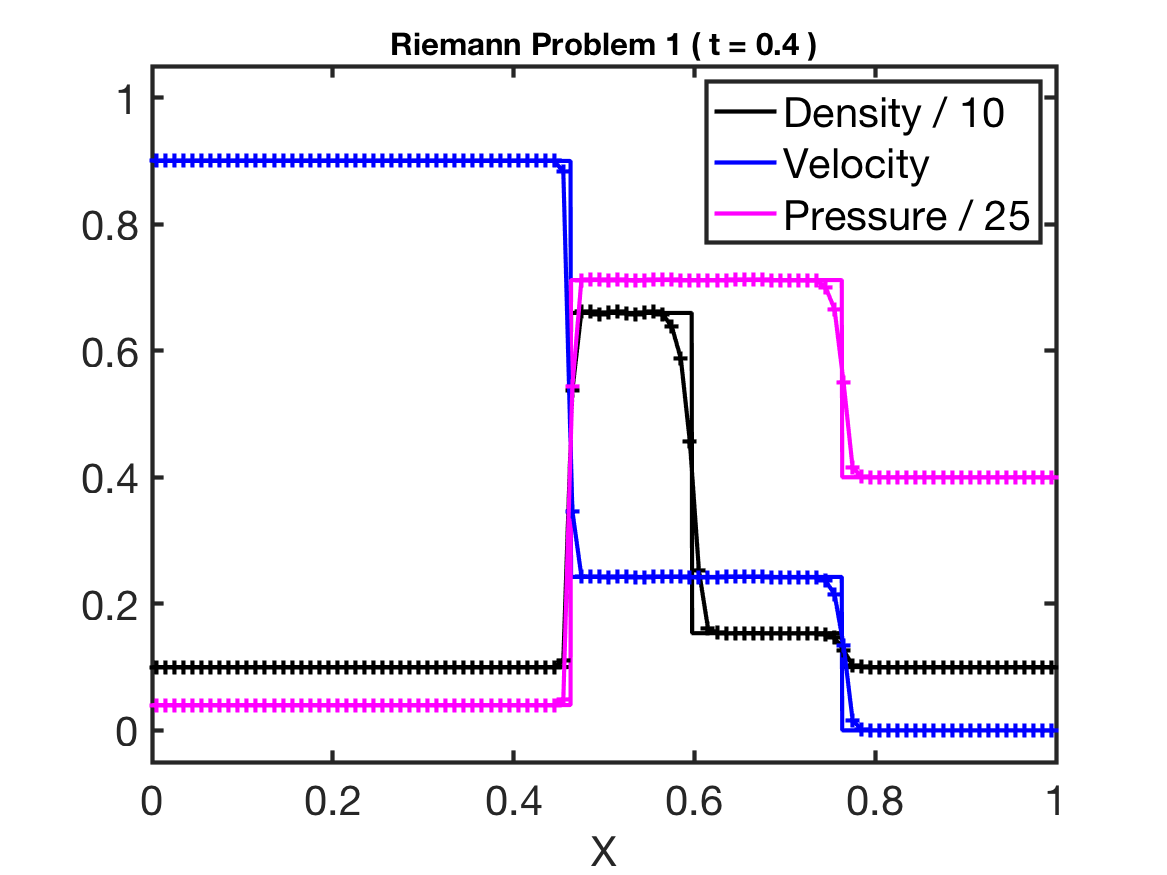
\includegraphics[width=18pc]{./Figures/MB2005_01_Astronum_2018}
  \end{minipage}\hspace{0.5pc}%
  \begin{minipage}{18pc}
    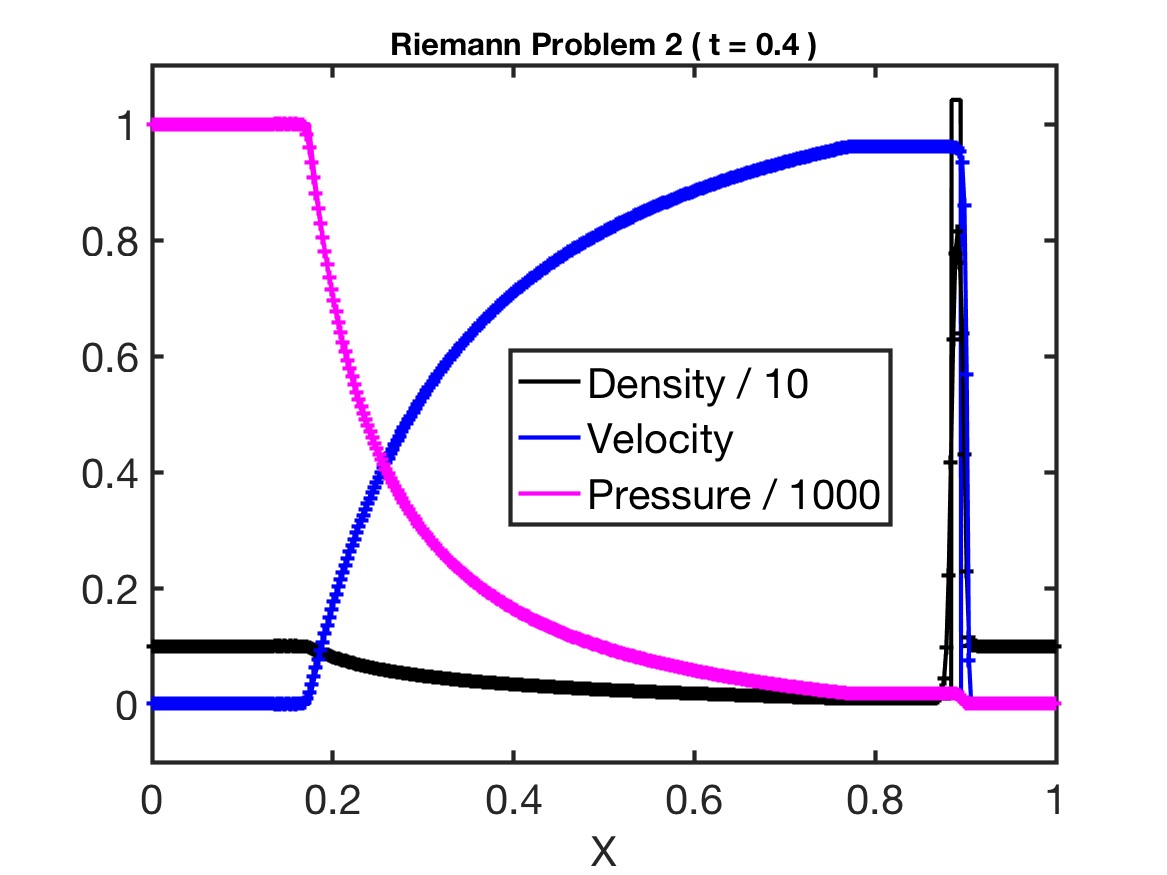
\includegraphics[width=18pc]{./Figures/MB2005_04_Astronum_2018}
  \end{minipage}
  \caption{\label{fig:RelativisticHydro}Results from solving the SR Euler equations with \thornado.  Riemann problem~1 (left panel) was solved using $100$ elements, while Riemann problem~2 was solved using $400$ elements.  The numerical and exact solutions are plotted with plusses and solid lines, respectively.}
\end{figure}

Again, the main features of the exact solution are captured with the DG method implemented in \thornado.  
For Riemann problem~1, we observe some oscillations in the density profile between the leftmost shock and the contact discontinuity located around $x^{1}=0.6$.  
For Riemann problem~2, the maximum density in the thin density shell between the shock and the contact discontinuity is significantly lower for the numerical solution than the exact solution.  
This is due to a combination of limited spatial resolution and the action of the slope limiter.  
We used $C_{\TCI}=0.03$ in both tests in this section.  
We have found the agreement with the exact solution to improve for larger values of $C_{\TCI}$, but at the expense of somewhat more oscillatory results.  

\section{Summary and outlook}

We have presented preliminary algorithm details and numerical results for solvers of the non-relativistic and special relativistic Euler equations of gas dynamics as implemented in the {\bf t}oolkit for {\bf h}igh-{\bf or}der {\bf n}eutrino-r{\bf ad}iation hydr{\bf o}dynamics (\thornado).  
The spatial discretization is based on the DG method and the ODEs resulting from this discretization are integrated in time using SSP-RK methods.  
We employ a spectral-type nodal collocation DG approximation based on Legendre-Gauss points for interpolation and numerical quadrature evaluation \cite{bassi_etal_2013}.  
This choice simplifies expressions for the semi-discretized equations, especially when applied to problems involving curvilinear coordinates encoded in a metric (e.g., in numerical relativity).  
Results from a suite of tests in one and two spatial dimensions --- including problems with strong shocks --- demonstrate reliable performance of the implementation.  
The accuracy of \thornado\ on three shock tests (Sod shock tube \cite{sod_1978}, Sedov-Taylor blast wave \cite{sedov_1959}, and Shu-Osher shock tube \cite{shuOsher_1989}) is qualitatively similar to that of the well-established CCSN simulation code \chimera\ \cite{bruenn_etal_2018}, which is based on the PPM finite volume method \cite{colellaWoodward_1984}.  
Two tests in spherical symmetry (standing accretion shock \cite{blondin_etal_2003} and Yahil-Lattimer collapse \cite{yahilLattimer_1982,yahil_1983}) demonstrate the DG method's ability to handle conditions relevant to CCSN simulations.  
We will present a more in-depth analysis of the performance of \thornado\ on these (and related) problems in a future study.  

The performance of the DG algorithm is sensitive to limiting of the polynomial representation.  
The combination of a TVD-type limiter (e.g., \cite{cockburnShu_1998}) and the troubled-cell indicator of \cite{fuShu_2017} seems to give satisfactory results for a range of problems.  
However, in our experience, the optimal value for the indicator threshold $C_{\TCI}$ seems to vary with the specific problem, and further investigation is needed to determine if there exists an optimal value suitable for CCSN simulations.  
Along these lines of investigation, it would also be interesting to explore and compare the use of the {\it a posteriori} subcell limiting approach in \cite{dumbser_etal_2014,fambri_etal_2018} with our current approach.  

Ongoing and planned near-future work within \thornado\ include coupling to solvers for two-moment neutrino transport, extensions to accommodate nuclear equations of state, general relativity within the conformal flatness approximation, and deployment within an adaptive mesh refinement framework.  
We hope to report on progress in these directions in the near future.  

\ack Eirik Endeve and Anthony Mezzacappa acknowledge support from the NSF Gravitational Physics Program (NSF-GP 1505933 and 1806692).

\section*{References}
\begin{thebibliography}{36}
  \bibitem{bassi_etal_2013} Bassi F, Franchina N, Ghidoni A and Rebay S 2013 {\it Int. J. Numer. Meth. Fluids} {\bf 71} 1322
  \bibitem{blondin_etal_2003} Blondin J M, Mezzacappa A and DeMarino C 2003 {\it ApJ} {\bf 584} 980
  \bibitem{brennerScott_2008} Brenner S C and Scott L R 2008 {\it The Mathematical Theory of Finite Element Methods} Springer
  \bibitem{bruenn_etal_2018} Bruenn S W {\it et al} {\it Preprint} arXiv:1809.05608
  \bibitem{cockburnShu_1998} Cockburn B and Shu C-W 1998 {\it JCP} {\bf 141} 199
  \bibitem{cockburnShu_2001} Cockburn B and Shu C-W 2001 {\it Journal of Scientific Computing} {\bf 16} 173
  \bibitem{colellaWoodward_1984} Colella P and Woodward P 1984 {\it JCP} {\bf 54} 174
  \bibitem{dumbser_etal_2014} Dumbser M, Zanotti O, Loub{\`e}re R and Diot S 2014 {\it JCP} {\bf 278} 47
  \bibitem{fambri_etal_2018} Fambri F, Dumbser M, K{\"o}ppel S, Rezzolla L and Zanotti O 2018 {\it MNRAS} {\bf 477} 4543
  \bibitem{fuShu_2017} Fu G and Shu C-W 2017 {\it JCP} {\bf 347} 305
  \bibitem{harten_etal_1983} Harten A, Lax P D and Van Leer B 1983 {\it SIAM~Review} {\bf 25} 35
  \bibitem{hesthavenWarburton_2008} Hesthaven J S and Warburton T 2008 {\it Nodal discontinuous Galerkin methods: Algorithms, analysis and applications} Springer
  \bibitem{klockner_etal_2009} Kl{\"o}ckner A, Warburton T, Bridge J and Hesthaven J S 2009 {\it JCP} {\bf 228} 7863
  \bibitem{landauLifshitz_1979} Landau L D and Lifshitz E M 1979 {\it Fluid Mechanics} Pergamon
  \bibitem{liskaWendroff_2003} Liska R and Wendroff B 2003 {\it SIAM J. Sci. Comput.} {\bf 25} 3
  \bibitem{martiMuller_2003} Mart{\'i} J M and M{\"u}ller E 2003 {\it Living Rev. Relativ.} {\bf 6} 7
  \bibitem{mcnally_etal_2012} McNally C, Lyra W and Passy J-C 2012 {\it ApJS} {\bf 201} 18
  \bibitem{mignoneBodo_2005} Mignone A and Bodo G 2005 {\it MNRAS} {\bf 364} 126
  \bibitem{muller_2016} M{\"u}ller B 2016 {\it PASA} {\bf 33} 1
  \bibitem{qin_etal_2016} Qin T, Shu C-W and Yang Y 2016 {\it JCP} {\bf 315} 323
  \bibitem{radiceRezzolla_2011} Radice D and Rezzolla L 2011 {\it Phys. Rev. D} {\bf 84} 024010
  \bibitem{remacle_etal_2003} Remacle J-F, Flaherty J E and Shephard M S 2003 {\it SIAM~Review} {\bf 45} 53
  \bibitem{schaal_etal_2015} Schaal K, Bauer A, Chandrashekar P R{\"u}diger P, Klingenberg C and Springel V 2015 {\it MNRAS} {\bf 453} 4278
  \bibitem{sedov_1959} Sedov L I 1959 {\it Similarity and Dimensional Methods in Mechanics} Academic Press
  \bibitem{shuOsher_1988} Shu C-W and Osher S 1988 {\it JCP} {\bf 77} 439
  \bibitem{shuOsher_1989} Shu C-W and Osher S 1989 {\it JCP} {\bf 83} 32
  \bibitem{shu_2016} Shu C-W 2016 {\it JCP} {\bf 316} 598
  \bibitem{sod_1978} Sod G A 1978 {\it JCP} {\bf 27} 1
  \bibitem{teukolsky_2016} Teukolsky S A 2016 {\it JCP} {\bf 312} 333
  \bibitem{toro_etal_1994} Toro E F, Spruce M and Speares W 1994 {\it Shock Waves} {\bf 4} 25
  \bibitem{toro_1999} Toro E F 1999 {\it NUMERICA: A Library of Source Codes for Teaching, Research and Applications}
  \bibitem{wilson_etal_1996} Wilson J R, Mathews G J and Marronetti P 1996 {\it Phys. Rev. D} {\bf 54} 1317
  \bibitem{wuTang_2015} Wu K and Tang H 2015 {\it JCP} {\bf 298} 539
  \bibitem{yahilLattimer_1982} Yahil A and Lattimer J M 1982 {\it Supernovae: A Survey of Current Research} Reidel
  \bibitem{yahil_1983} Yahil A 1983 {\it ApJ} {\bf 265} 1047
  \bibitem{zhangShu_2010} Zhang X and Shu C-W 2010 {\it JCP} {\bf 229} 8918
\end{thebibliography}

\end{document}


